\chapter{Экспериментальное исследование}

Настоящая глава описывает экспериментальную часть работы как единый блок: постановка задачи, методика, реализация и результаты. Изложение организовано вокруг двух самостоятельных эмпирических результатов. Первый~--- диагностика и закрытие <<setup-gap>> на этапе персонального последовательного скорера, в ходе которой воспроизведён яндексовский SASRec-бейзлайн на YAMBDA и выявлена доменная особенность повторного потребления в музыке (раздел~\ref{sec:ch3:scorer}). Второй~--- сравнение четырёх обучаемых групповых агрегаторов поверх замороженного скорера и проверка центральной гипотезы работы о преимуществе audio-aware attention над ID-based attention (разделы~\ref{sec:ch3:group-method}~и~\ref{sec:ch3:results}).

Методологическая рамка работы~--- двухуровневая: фиксированный sequential per-user скорер плюс обучаемый групповой агрегатор. Эта рамка соответствует индустриальному two-stage retrieval-rerank сетапу, в котором сильный персональный ранжировщик уже обучен и переиспользуется поверх него тонкая агрегационная надстройка. Такое разделение даёт чистую ablation вклада агрегационного механизма и снимает значительную долю компьюта при сравнении большого числа методов.

\section{Постановка задачи и гипотеза}\label{sec:ch3:setup}

\subsection{Задача групповых рекомендаций}

Пусть $\mathcal{U} = \{u_1, \ldots, u_{|\mathcal{U}|}\}$~--- множество пользователей, $\mathcal{I}$~--- каталог музыкальных треков. История взаимодействий пользователя $u$ представляется упорядоченной во времени последовательностью прослушиваний
\begin{equation}
    \mathcal{S}_u = \left( (i_1^{(u)}, t_1^{(u)}), \ldots, (i_{n_u}^{(u)}, t_{n_u}^{(u)}) \right), \qquad t_1^{(u)} < \ldots < t_{n_u}^{(u)},
\end{equation}
а персональный последовательный скорер $f_\theta$ с параметрами $\theta$ по истории $\mathcal{S}_u^{(<t)}$ оценивает релевантность каждого трека $i \in \mathcal{I}$ на следующем шаге:
\begin{equation}
    \hat{s}_{u, i} = f_\theta\!\left( \mathcal{S}_u^{(<t)}, i \right) \in \mathbb{R}.
\end{equation}

Под группой пользователей $G = \{u_1, \ldots, u_{|G|}\} \subseteq \mathcal{U}$ понимается эфемерная группа, сформированная на короткий промежуток времени совместного потребления музыки (посетители заведения, участники мероприятия). Задача групповых рекомендаций состоит в построении списка $\mathrm{Rec}_K(G)$ длины $K$, который в совокупности удовлетворяет всех членов группы:
\begin{equation}
    \mathrm{Rec}_K(G) = \underset{i \in \mathcal{C}_G}{\mathrm{argtop}\text{-}K}\, \hat{s}_{G, i},
    \qquad
    \hat{s}_{G, i} = \mathcal{A}\!\left( \left\{ \hat{s}_{u, i} \right\}_{u \in G}, \, \mathbf{a}_i, \, \{\bar{\mathbf{a}}_u\}_{u \in G} \right),
\end{equation}
где $\mathcal{A}$~--- функция группового агрегатора, $\mathbf{a}_i \in \mathbb{R}^{d_a}$~--- аудиоэмбеддинг трека~$i$, предоставляемый датасетом YAMBDA~\cite{yambda2025}, $\bar{\mathbf{a}}_u \in \mathbb{R}^{d_a}$~--- аудиопрофиль пользователя, полученный усреднением аудиоэмбеддингов треков из его обучающей истории, $\mathcal{C}_G \subseteq \mathcal{I}$~--- кандидатное множество группы, образованное объединением персональных топ-$K$ кандидатов её членов.

Эфемерность группы и отсутствие реальных групп в открытых датасетах~\cite{cao2018agree, sankar2020groupim} определяют две методологические особенности постановки. Во-первых, групповые эмбеддинги не могут быть обучены на персистентных группах~--- агрегатор должен оперировать индивидуальными представлениями членов. Во-вторых, группы формируются синтетически из индивидуальных профилей пользователей датасета; процедура их синтеза описана в подразделе~\ref{subsec:ch3:groups-synthesis}.

\subsection{Двухуровневая схема: замороженный скорер плюс обучаемый агрегатор}\label{subsec:ch3:framework}

Центральная методологическая рамка работы~--- декомпозиция задачи на два уровня:

\begin{enumerate}
    \item \textbf{Персональный уровень.} Для каждого пользователя $u \in G$ независимо вычисляются персональные скоры $\hat{s}_{u, i} = f_\theta(\mathcal{S}_u^{(<t)}, i)$ фиксированной моделью последовательного ранжирования. Параметры $\theta$ обучаются один раз на индивидуальных next-item задачах и далее не модифицируются.
    \item \textbf{Групповой уровень.} Обучаемый агрегатор $\mathcal{A}_\psi$ с параметрами $\psi$ преобразует множество персональных скоров $\{\hat{s}_{u, i}\}_{u \in G}$ в групповую оценку $\hat{s}_{G, i}$. Обучаются только параметры~$\psi$; скорер $f_\theta^\ast$ остаётся замороженным.
\end{enumerate}

Такое разделение методологически продумано и согласуется с распространённой в индустрии двухэтапной схемой <<retrieval~$\to$~rerank>>~\cite{covington2016youtube, volokitin2023yandex}: сильный персональный ранжировщик уже обучен на большом объёме индивидуальных данных и переиспользуется в групповом сценарии без дообучения, а тонкая агрегационная надстройка обучается на синтетических группах с существенно меньшими вычислительными затратами. Полный end-to-end fine-tune скорера под групповую задачу~--- естественное продолжение, обсуждаемое в разделе~\ref{sec:ch3:limitations} как направление развития. В основной таблице сравнения замороженный скорер обеспечивает (а)~однозначную атрибуцию различий между методами агрегационному механизму, (б)~возможность кэширования персональных скоров и многократного переиспользования кэша всеми сравниваемыми агрегаторами, (в)~совместимость с типичным production-ландшафтом, где переобучение базового ранжировщика стоит на порядки дороже обучения rerank-надстройки.

\subsection{Предлагаемая модификация: audio-aware attention}\label{subsec:ch3:proposal}

Существующие attention-агрегаторы для эфемерных групп~--- AGREE~\cite{cao2018agree} и GroupIM~\cite{sankar2020groupim}~--- оперируют исключительно обучаемыми ID-эмбеддингами пользователей и треков. В музыкальном домене такая привязка к ID имеет два недостатка: качество обучаемых эмбеддингов быстро деградирует на хвосте каталога, а для треков, не встречавшихся в истории членов группы, ID-сигнал в принципе отсутствует.

Аудиоэмбеддинги YAMBDA дают альтернативный непрерывный сигнал, доступный для любого трека каталога независимо от частоты его прослушиваний. На этом наблюдении строится предложенное в работе семейство audio-aware агрегаторов: ID-эмбеддинг $\mathbf{e}_i$ в attention-формуле заменяется на аудиоэмбеддинг $\mathbf{a}_i$, а ID-эмбеддинг пользователя $\mathbf{e}_u$~--- на аудиопрофиль $\bar{\mathbf{a}}_u$. Реализованы две архитектурные точки этого семейства:

\begin{itemize}
    \item \textbf{Audio-AGREE}~--- прямой аналог item-aware attention AGREE с заменой $(\mathbf{e}_u, \mathbf{e}_i)$ на $(\bar{\mathbf{a}}_u, \mathbf{a}_i)$. Вес члена группы вычисляется обучаемой скоринговой функцией $\phi_\psi$ поверх конкатенации аудиопрофиля пользователя и аудиоэмбеддинга кандидата.
    \item \textbf{Group Cross-Attention}~--- многоголовое scaled dot-product cross-attention, в котором кандидат $\mathbf{a}_i$ используется как запрос (query), аудиопрофили членов группы~--- как ключи (keys). Это естественное обобщение Audio-AGREE: однопроекционный MLP-логит заменяется на $H$ голов dot-product attention.
\end{itemize}

Точные определения архитектур приведены в подразделе~\ref{subsec:ch3:aggregators}. Принципиально, что обе предложенные модификации сохраняют единый контракт агрегационной формулы $\hat{s}_{G, i} = \sum_{u \in G} \alpha_{u, i} \hat{s}_{u, i}$~--- веса по членам группы суммируются в единицу, и итоговая оценка остаётся выпуклой комбинацией персональных скоров замороженного скорера. Это обеспечивает чистоту ablation между ID-вариантом (AGREE, GroupIM) и audio-вариантом (Audio-AGREE, Group Cross-Attention): различие сводится к замене источника сигнала в attention-логите при одинаковом фрейме агрегации.

\subsection{Гипотеза}\label{subsec:ch3:hypothesis}

Эксперимент проверяет центральную гипотезу работы:

\begin{quote}
\textbf{H1.} При фиксированном персональном последовательном скорере на YAMBDA-50m audio-aware attention-агрегаторы (Audio-AGREE, Group Cross-Attention) превосходят ID-based attention-агрегаторы (AGREE, GroupIM) по групповому NDCG@10/20 на синтетических случайных группах.
\end{quote}

В качестве вспомогательных точек сравнения в основной таблице приводятся классические необучаемые стратегии~--- среднее (Average), стратегия наименьшего недовольства (Least Misery) и максимального удовольствия (Max Pleasure)~\cite{cao2018agree}. Они выполняют роль <<тривиальных>> бейзлайнов, относительно которых оценивается полезность обучаемой надстройки в принципе. Дополнительные постановки~--- гомогенные / гетерогенные группы по сходству вкусов, cold-start срез по доле редких треков, метрики справедливости и разнообразия (Jain@K, Disagreement@K)~--- сформулированы методически и вынесены в раздел~\ref{sec:ch3:limitations} как направления развития исследования.

\section{Данные: YAMBDA-50m}\label{sec:ch3:data}

\subsection{Характеристики датасета}\label{subsec:ch3:data-overview}

В качестве источника данных используется YAMBDA~\cite{yambda2025}~--- открытый датасет взаимодействий пользователей с музыкальным каталогом, опубликованный командой Яндекс Музыки в 2025~году. Датасет содержит около $4{,}79 \cdot 10^9$ событий взаимодействий, $|\mathcal{U}| \approx 10^6$ уникальных пользователей и $|\mathcal{I}| \approx 9{,}4 \cdot 10^6$ уникальных треков. Каждое событие представлено кортежем $(u, i, t, \mathrm{type}, \mathrm{is\_organic})$, где $\mathrm{type}$~--- тип взаимодействия (прослушивание, лайк, дизлайк, пропуск), а $\mathrm{is\_organic} \in \{0, 1\}$~--- флаг, отделяющий органические действия пользователя от событий, инициированных рекомендательной системой платформы.

Для каждого трека $i \in \mathcal{I}$ в датасете предоставлен предобученный аудиоэмбеддинг $\mathbf{a}_i \in \mathbb{R}^{d_a}$, полученный внутренней моделью Яндекса. Семантическая интерпретация осей эмбеддинга, а также метаданные треков (исполнитель, жанр, год выпуска, текстовое описание) в открытой версии датасета отсутствуют: идентификаторы $i$ являются анонимизированными внутренними кодами и не сопоставимы с публичными музыкальными базами. YAMBDA (2025) принципиально отделяется от датасета \emph{Yandex Music Event} (2019)~\cite{abbattista2024sequential}: последний содержит около $4{,}77 \cdot 10^7$ событий, не включает аудиоэмбеддинги и не пригоден для задач, рассматриваемых в настоящей работе.

\paragraph{Выбор flavor.} В работе используется единственный flavor~--- \texttt{50m}, содержащий первые $4{,}78 \cdot 10^7$ событий полного датасета. Использование полного flavor (\texttt{5b}) исключено вычислительными ограничениями: эксперименты выполняются в среде Google Colab с доступом к графическим ускорителям A100 (40~GB) и G4 (95~GB RAM) на ограниченные временные сессии. Принципиально важная особенность YAMBDA, не очевидная из названий: \emph{flavor отражает число событий, а не пользователей}~--- \texttt{50m} соответствует $50 \cdot 10^6$ событий, что после фильтрации даёт лишь около 9~тысяч уникальных пользователей. Это объясняется длинными музыкальными историями (медиана~--- $\sim\!1800$ прослушиваний на пользователя) и накладывает ограничения на статистическую мощность последующих сравнений, обсуждаемые в разделах~\ref{sec:ch3:results}~и~\ref{sec:ch3:limitations}.

\subsection{Фильтрация событий}\label{subsec:ch3:filter}

К сырому потоку событий flavor \texttt{50m} применяется последовательность шагов фильтрации, согласованная со стандартной практикой YAMBDA~\cite{yambda2025}.

\textbf{Тип взаимодействий.} В качестве позитивных взаимодействий рассматриваются исключительно события прослушивания с долей проигрывания не менее~50\% длительности трека ($\mathtt{played\_ratio\_pct} \geq 50$). Этот порог совпадает с константой \texttt{TRACK\_LISTEN\_THRESHOLD} официального API YAMBDA. Пропуски, дизлайки и лайки в обучении и в построении персональных скоров не используются: первые два несут отрицательный сигнал, третьи на порядки реже прослушиваний и не дают достаточной статистики для последовательного моделирования. Распределение \texttt{played\_ratio\_pct} среди событий прослушивания сильно скошено к 100\% (медиана и 90-й процентиль равны 100), что подтверждает корректность порога~50\%: фильтр отсекает короткие <<пробные>> прослушивания, оставляя содержательное потребление.

После фильтра по типу остаётся $2{,}94 \cdot 10^7$ событий, 9{,}209 уникальных пользователей и 631{,}003 уникальных трека.

\textbf{Порог популярности трека.} На отфильтрованной выборке применяется порог минимальной популярности трека: $\mathtt{min\_pop} \geq 5$ прослушиваний за период наблюдения. Этот шаг сокращает каталог с 631{,}003 до 276{,}305 уникальных треков ($-56\%$), теряя при этом лишь $\sim\!2{,}1\%$ событий и 14~пользователей из 9{,}209 (у которых вся история состояла исключительно из редких треков). Распределение популярности треков с подсветкой эффекта фильтра приведено на рис.~\ref{fig:item-pop-zipf}.

\textbf{Порядок применения шагов.} Фильтр \texttt{min\_pop} применяется \emph{до} построения временного сплита и перенумерации идентификаторов треков ($\mathtt{item\_id} \to \mathtt{idx}$). Альтернативный порядок (применить порог после сплита) допускает попадание в обучающую выборку редких треков, которые после перенумерации становятся отсутствующими в валидации и тесте, что нарушает согласованность embedding-таблицы между обучением и инференсом. Канонический pipeline зафиксирован как \texttt{load $\to$ filter\_listens $\to$ filter\_min\_popularity $\to$ build\_item\_id\_to\_idx $\to$ apply\_item\_remap $\to$ global\_temporal\_split}.

\textbf{Повторные прослушивания.} В отличие от ряда работ, агрегирующих повторные прослушивания одного и того же трека пользователем в одно взаимодействие, в настоящей работе повторные прослушивания сохраняются. Это обусловлено спецификой музыкального домена: повторное потребление является существенной составляющей пользовательского поведения~\cite{abbattista2024sequential, greer2025beyond}. Сохранение повторов оказывается принципиально важно и для построения eval-протокола~--- этому посвящён подраздел~\ref{subsec:ch3:setup-gap} с диагностикой setup-gap.

\textbf{Характеристики истории.} После фильтрации медиана длины истории пользователя составляет $\sim\!1{,}760$ прослушиваний, 95-й процентиль~--- $\sim\!11{,}200$, максимум~--- $\sim\!27{,}000$. Гистограмма распределения длин историй с подсветкой выбранного \texttt{max\_seq\_len}~=~200 и медианы приведена на рис.~\ref{fig:history-hist}. Это распределение содержательно отличается от классических movie/book-датасетов (MovieLens, Goodreads) с десятками или сотнями взаимодействий на пользователя и определяет ряд решений, обсуждаемых далее: выбор $\mathtt{max\_seq\_len}$, режим маскирования истории при ранжировании, выбор негативных примеров.

\begin{figure}[ht]
    \centering
    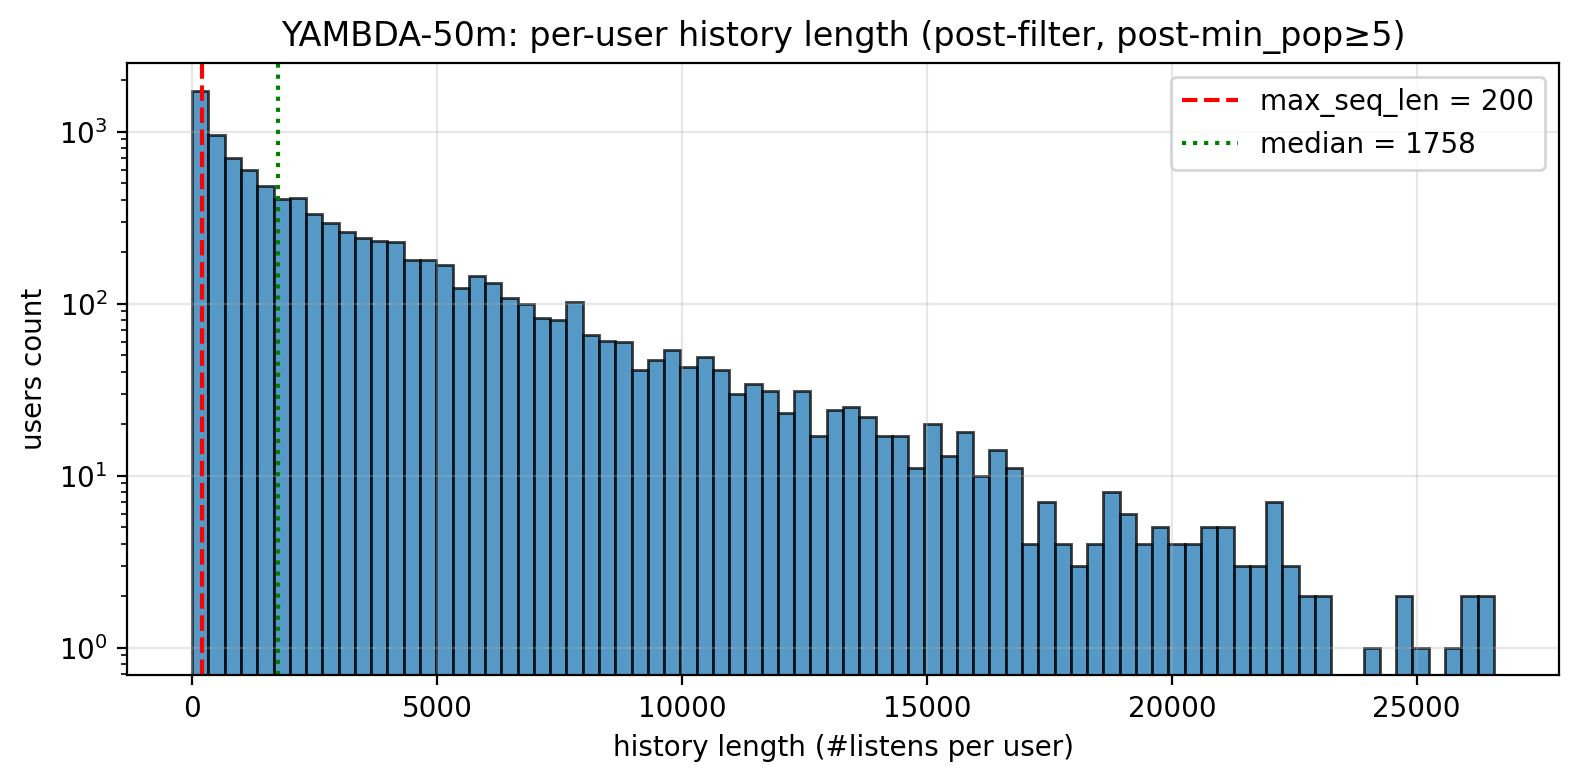
\includegraphics[width=0.85\textwidth]{graphics/history_length_hist.png}
    \caption{Распределение длины пользовательских историй после фильтрации (YAMBDA-50m, listen+, \texttt{min\_pop}~$\geq$~5). Log-шкала по оси~$y$. Вертикальные линии~--- медиана ($\sim\!1{,}760$) и выбранное значение \texttt{max\_seq\_len}~=~200.}
    \label{fig:history-hist}
\end{figure}

\begin{figure}[ht]
    \centering
    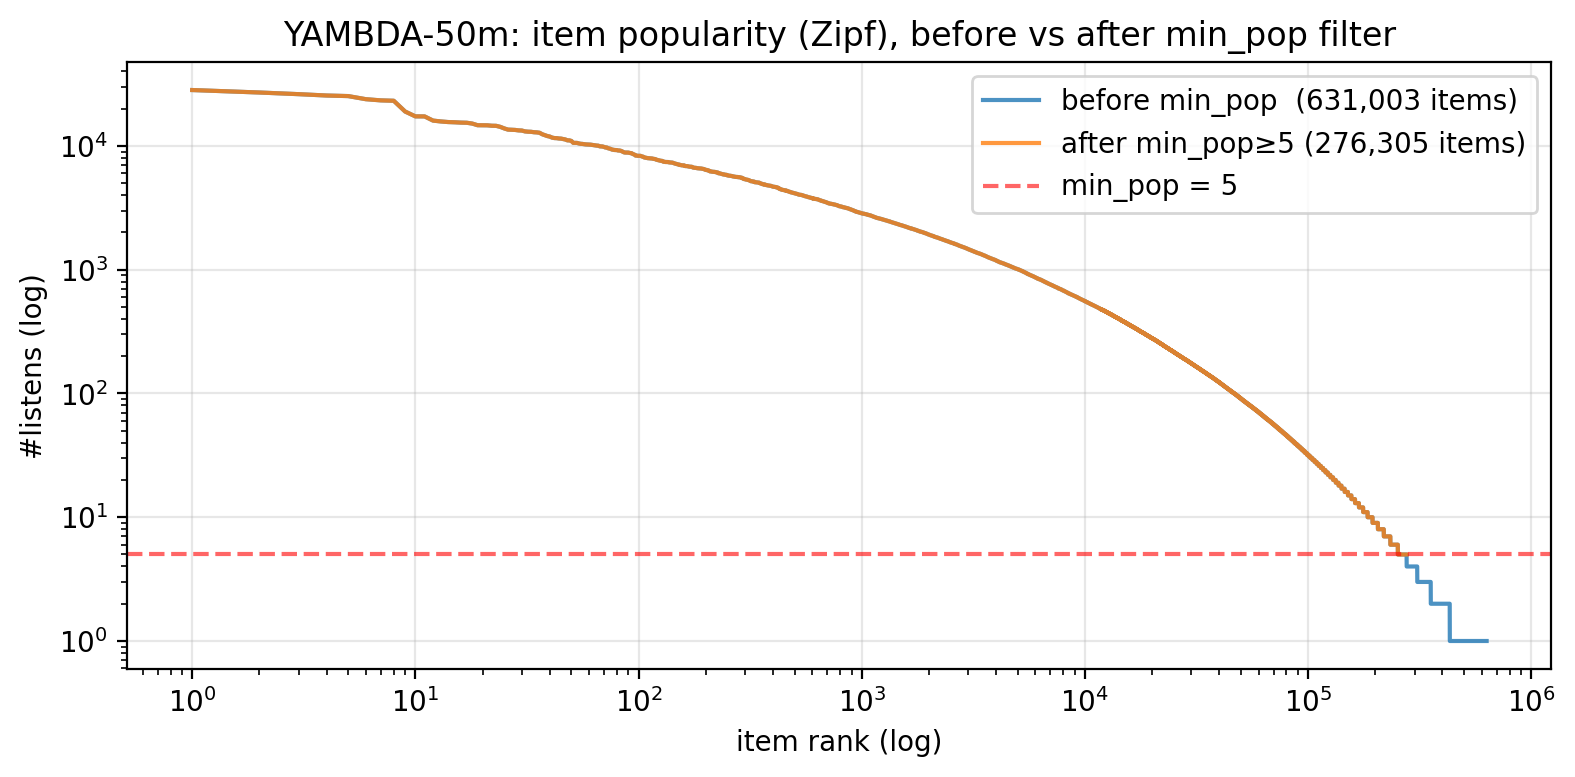
\includegraphics[width=0.85\textwidth]{graphics/item_popularity_zipf.png}
    \caption{Распределение популярности треков (log-log) до и после фильтра \texttt{min\_pop}~$\geq$~5. Фильтр срезает только хвост каталога ($631\mathrm{k} \to 276\mathrm{k}$ треков), не затрагивая голову распределения.}
    \label{fig:item-pop-zipf}
\end{figure}

\subsection{Временной сплит}\label{subsec:ch3:split}

В качестве протокола разделения данных на обучающую, валидационную и тестовую выборки используется \emph{глобальный временной сплит} (global timeline split, GTS)~\cite{yambda2025, volokitin2023yandex}. Пусть $T = 26 \cdot 10^6$~--- общая временная протяжённость датасета (в условных единицах YAMBDA, привязанных к минимальной временной шкале источника). Выбираются две точки $t_{\mathrm{train}} = T - \tau_{\mathrm{val}} - \tau_{\mathrm{test}} - \delta$ и $t_{\mathrm{val}} = T - \tau_{\mathrm{test}}$, где $\tau_{\mathrm{val}} = \tau_{\mathrm{test}} = 86{,}400$ соответствует одному календарному дню, а $\delta = 1{,}800$~--- защитный зазор (gap), исключающий пограничные эффекты. Для каждого пользователя $u$:
\begin{itemize}
    \item обучающая выборка содержит события $\{ (i, t) \in \mathcal{S}_u : t < t_{\mathrm{train}} \}$;
    \item валидационная~--- $\{ (i, t) \in \mathcal{S}_u : t_{\mathrm{train}} + \delta \leq t < t_{\mathrm{val}} \}$;
    \item тестовая~--- $\{ (i, t) \in \mathcal{S}_u : t \geq t_{\mathrm{val}} \}$.
\end{itemize}
Точкой отсечки теста является $t_{\mathrm{test}} = 25{,}913{,}600$. Распределение пользователей по сегментам после применения сплита~--- $9{,}194 / 4{,}596 / 4{,}576$ для train/val/test соответственно (валидация и тест ограничены пользователями, имеющими хотя бы одно событие в обучающей выборке). Поведенческий характер потока событий (распределение по часам, недельная модуляция, согласованность распределений между train/val/test) визуализирован на рис.~\ref{fig:gts-timeline}.

\begin{figure}[ht]
    \centering
    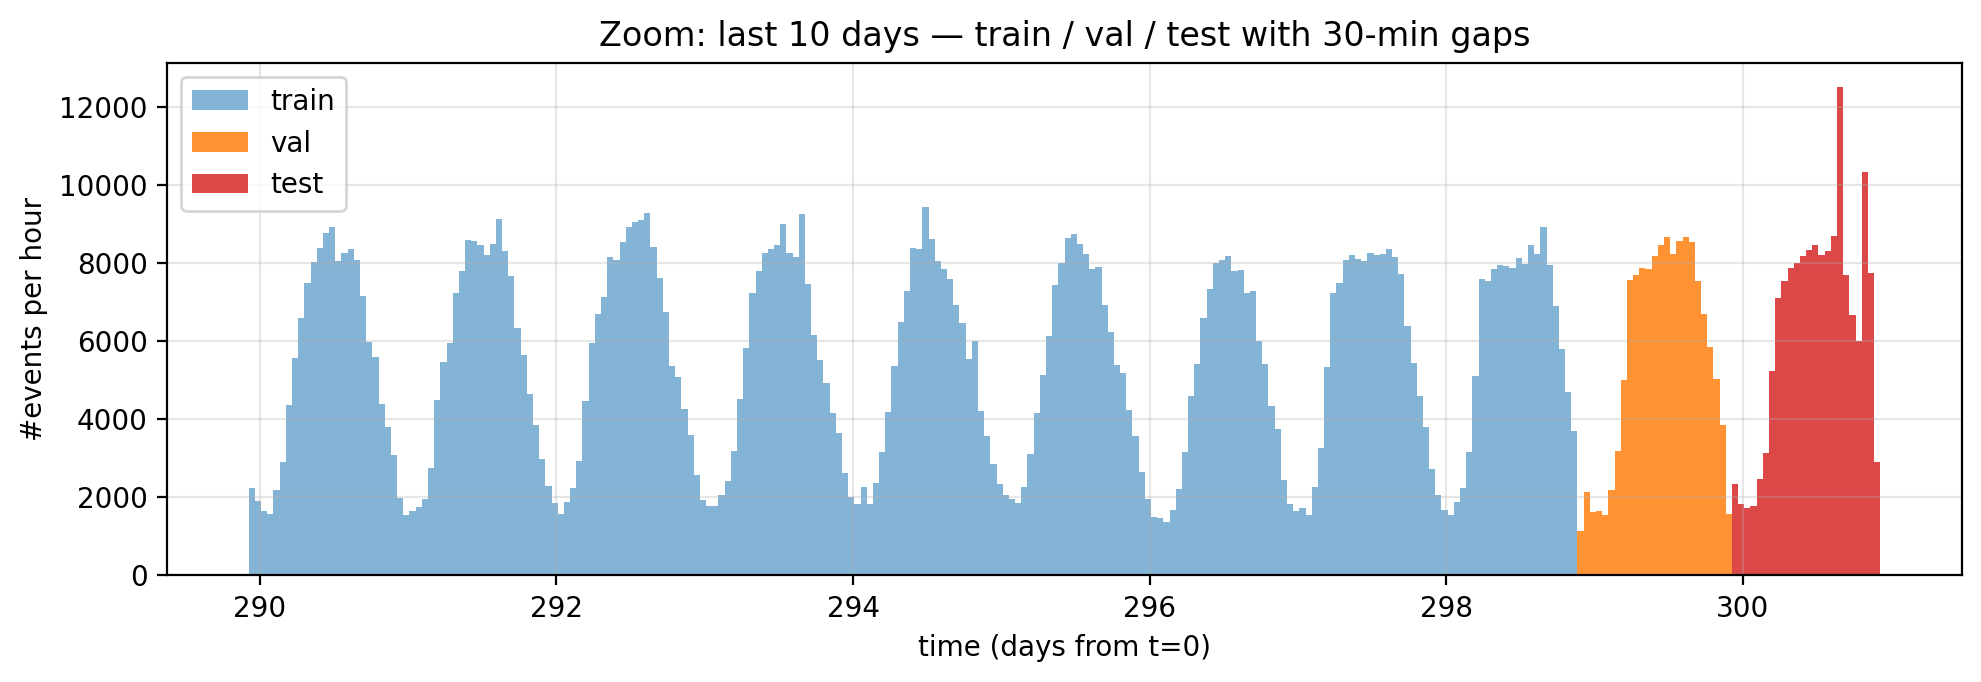
\includegraphics[width=0.85\textwidth]{graphics/gts_timeline_zoom.png}
    \caption{Глобальный временной сплит, увеличенное окно на границе train/val/test. Видна суточная модуляция активности и согласованность распределений между сегментами (отсутствие distribution shift). Защитные зазоры в 30~минут не разрешаются на часовых корзинах гистограммы.}
    \label{fig:gts-timeline}
\end{figure}

Выбор GTS вместо распространённой схемы leave-one-out обусловлен тремя соображениями~\cite{petrov2022bert4rec_replicability, volokitin2023yandex}. Во-первых, GTS не нарушает каузальность во времени: при обучении модель не имеет доступа ни к одному событию из будущего ни одного пользователя, что воспроизводит реальную production-постановку. Во-вторых, GTS корректно учитывает популярные тренды (выход новых треков, сезонные эффекты), оценивая способность модели обобщать на действительно новые элементы каталога. В-третьих, исследования воспроизводимости показывают, что leave-one-out склонен переоценивать качество последовательных моделей за счёт скрытых утечек. Длительность валидационного и тестового окон в 1~день выбрана компромиссом между статистической мощностью оценок (требование $\geq 10^3$ пользователей в каждом сегменте~--- в нашем случае пройдено с запасом) и сохранением основного объёма данных в обучении.

\subsection{Аудиоэмбеддинги: размерность, покрытие, извлечение subset}\label{subsec:ch3:audio}

Аудиоэмбеддинги YAMBDA хранятся в Hugging Face Hub в виде parquet-файла $\texttt{embeddings.parquet}$ ($\sim\!14$~GB, $7{,}721{,}749$ строк) с колонками $\mathtt{item\_id}$ (uint32), $\mathtt{embed}$ (большой массив double длины $d_a$) и $\mathtt{normalized\_embed}$ (то же, нормированный по $\ell_2$). Полная загрузка файла на Colab-диск возможна, но во-первых дорогостояща по времени, во-вторых~--- избыточна для нашей фильтрованной выборки в 276{,}305 треков. Поэтому реализована процедура извлечения subset:

\begin{enumerate}
    \item \textbf{Определение $d_a$ без загрузки данных.} Через \texttt{HfFileSystem} прочитан footer parquet-файла (несколько килобайт range-read из конца файла), оттуда извлечена схема и получено $d_a = 128$. Это позволило зафиксировать размерность аудио до закладки на компьют, без скачивания 14~GB.
    \item \textbf{Загрузка и фильтрация на Colab.} Полный $\texttt{embeddings.parquet}$ скачивается на сессионный диск, читается в \texttt{pyarrow.Table} в две колонки ($\mathtt{item\_id}$, $\mathtt{embed}$), фильтруется по $\mathtt{np.isin}(\mathtt{item\_id}, \mathtt{target\_ids})$ с целевыми идентификаторами из $\mathtt{item\_id\_to\_idx}$ настоящей работы, и сохраняется массивом \texttt{[n\_items + 1, 128]} типа \texttt{float32} ($\sim\!135$~MB), нулевая строка зарезервирована под PAD.
    \item \textbf{Покрытие.} Из 276{,}305 треков аудио доступно для 264{,}840 ($95{,}85\%$); 11{,}465 треков ($4{,}15\%$) аудио не имеют и сохраняются как нулевые строки в субсете. Анализ доли пропусков по квантилям популярности (медианная популярность отсутствующих в аудио треков~--- 15, присутствующих~--- 18; максимум популярности отсутствующих~--- 12{,}770, $p_{90} = 142$) показывает, что пропуски распределены по всему диапазону популярности, а не сосредоточены в хвосте. Это~--- эффект <<catalog drift>>: 4\% треков снимаются с раздачи по правам или удаляются между snapshot'ами датасета, без корреляции с активностью прослушивания.
\end{enumerate}

\textbf{Контракт по пропускам.} В audio-aware агрегаторах missing-кандидаты (нулевой $\mathbf{a}_i$) дают близкий к нулю вклад в attention-логит, что приводит к мягкому fallback на равномерный вес и эквивалентно усреднению персональных скоров по членам группы. Это естественная degradation без edge-case-обработки и совпадает с поведением ID-методов, которые на тех же missing-треках вообще не получают сигнала. Для пользовательских аудиопрофилей missing-треки исключаются из усреднения; пользователи, у которых вся история состоит исключительно из таких треков (вырожденный случай, не наблюдавшийся в данных), получают нулевой профиль с явным маркером невалидности.

\textbf{Аудиопрофиль пользователя.} Для каждого пользователя $u$ из обучающей части аудиопрофиль определяется как среднее аудиоэмбеддингов прослушанных треков:
\begin{equation}
    \bar{\mathbf{a}}_u = \frac{1}{|\mathcal{S}_u^{\mathrm{train, valid}}|} \sum_{j \in \mathcal{S}_u^{\mathrm{train, valid}}} \mathbf{a}_j,
\end{equation}
где $\mathcal{S}_u^{\mathrm{train, valid}}$~--- множество прослушанных пользователем треков из обучающего периода, для которых $\mathbf{a}_j \neq \mathbf{0}$ (то есть с доступным аудио). Использование исключительно обучающей истории, а не полной, исключает утечку информации из валидации и теста в audio-aware агрегатор.

\section{Персональный последовательный скорер}\label{sec:ch3:scorer}

Цель настоящего раздела~--- зафиксировать персональный последовательный скорер $f_\theta^\ast$, выступающий неизменным входом группового агрегатора. Раздел организован вокруг двух связанных результатов: во-первых, выбор архитектуры и режима обучения (подразделы~\ref{subsec:ch3:sasrec-arch}~и~\ref{subsec:ch3:scorer-train}); во-вторых, диагностика и закрытие <<setup-gap>>~--- разрыва между качеством исходно реализованного скорера ($\mathrm{NDCG@10} = 0{,}0117$) и яндексовским baseline на тех же данных ($\mathrm{NDCG@10} = 0{,}0742$), потребовавшая последовательного пересмотра ряда стандартных решений и завершившаяся доменным наблюдением о роли повторного потребления при ранжировании в музыке (подраздел~\ref{subsec:ch3:setup-gap}). Диагностика setup-gap подаётся в работе как самостоятельный методологический результат, а не как технический служебный этап: её ключевое наблюдение прямо опровергает молчаливо принятый в movie/book-литературе стандарт eval-протокола и имеет практические последствия для воспроизводимости в музыкальном домене.

\subsection{Архитектура: SASRec}\label{subsec:ch3:sasrec-arch}

В качестве архитектуры используется SASRec (Self-Attentive Sequential Recommendation)~\cite{sasrec2018}~--- трансформерная модель последовательных рекомендаций с каузальной маской самовнимания, ставшая де-факто стандартом в литературе по next-item-предсказанию~\cite{petrov2022bert4rec_replicability, gsasrec2023}. Реализация написана с нуля в \texttt{src/scorer/gsasrec.py} с прямой адаптацией к специфике задачи, без импорта из эталонной реализации yambda~\cite{yambda2025} или авторского репозитория gSASRec~\cite{gsasrec2023}; обоснование выбора и отказ от gBCE-функции потерь обсуждается в подразделе~\ref{subsec:ch3:setup-gap}. Общая схема архитектуры приведена на рис.~\ref{fig:sasrec-arch}.

\begin{figure}[ht]
    \centering
    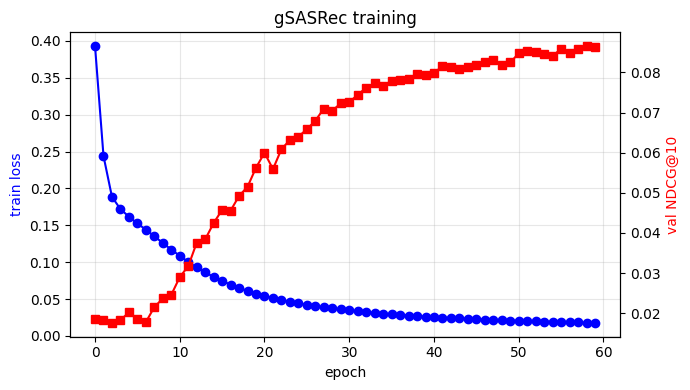
\includegraphics[width=0.75\textwidth]{graphics/sasrec_graph.png}
    \caption{Схема архитектуры SASRec~\cite{sasrec2018}: входная последовательность item-эмбеддингов с добавленными позиционными эмбеддингами проходит через стек блоков self-attention с каузальной маской и feed-forward подсетей; представление последнего токена используется для скоринга кандидатов через скалярное произведение с item-эмбеддингами.}
    \label{fig:sasrec-arch}
\end{figure}

\paragraph{Кодирование последовательности.} Для пользователя $u$ с историей $\mathcal{S}_u^{(<t)}$ берутся последние $L = \mathtt{max\_seq\_len} = 200$ прослушанных треков, представленные индексами $\mathtt{item\_idx} \in \{1, \ldots, |\mathcal{I}|\}$, нулевой индекс зарезервирован под PAD. Применяется \emph{левая} (\emph{prepend}) стратегия паддинга: при $|\mathcal{S}_u^{(<t)}| < L$ слева добавляются нули, наиболее свежее событие всегда занимает позицию $L - 1$. Позиционные индексы фиксированы как $0, 1, \ldots, L - 1$ безотносительно фактической длины истории. Такая конструкция позволяет извлекать представление последнего токена однообразно как \texttt{hidden[:, -1, :]} без \texttt{gather} по индексам реальных длин, что снимает целый класс ошибок с offsets/cumsum.

Эмбеддинги треков хранятся в обучаемой таблице $\mathbf{E} \in \mathbb{R}^{(|\mathcal{I}|+1) \times d}$ c $\mathtt{padding\_idx}=0$~--- нулевая строка инициализируется нулями и не обновляется при обучении. Позиционные эмбеддинги $\mathbf{P} \in \mathbb{R}^{L \times d}$~--- обучаемые. Входной тензор последовательности
\begin{equation}
    \mathbf{X} = \mathrm{Dropout}\!\left( \mathbf{E}[\mathbf{s}] + \mathbf{P} \right) \in \mathbb{R}^{B \times L \times d}
\end{equation}
подаётся в стек блоков \texttt{nn.TransformerEncoderLayer} с \texttt{batch\_first=True}, post-LN-конфигурацией и feed-forward-сетью с GELU-активацией.

\paragraph{Маскирование self-attention.} В каждом блоке применяется композиция двух масок: каузальная \texttt{causal\_mask = triu(ones, diag=1)}, запрещающая каждой позиции аттендиться на будущие, и пер-батч маска паддинга \texttt{key\_padding\_mask = (seq == 0)}, исключающая нулевые токены из множества ключей. Прямолинейная композиция через \texttt{src\_key\_padding\_mask}-аргумент \texttt{TransformerEncoder} приводит к корректному поведению для большинства пользовательских историй, однако создаёт скрытый артефакт для коротких историй ($|\mathcal{S}_u^{(<t)}| < L$): query-позиции в пад-зоне получают полностью замаскированный набор ключей (каузальный фильтр оставляет только пад-токены до текущей позиции, key-pad-маска их обнуляет), что даёт $\mathrm{softmax}(-\infty) = \mathrm{NaN}$. Через residual-связи NaN распространяется до правой границы последовательности (позиции $L-1$) и в конечном счёте до выхода \texttt{score()}.

Эффект латентный (синтетика на полностью заполненных историях работает корректно) и был обнаружен только на стадии построения кэша скоров (раздел~\ref{subsec:ch3:cache}): из 9{,}194 обучающих пользователей у 1{,}222 ($13{,}3\%$) кэш оказался полностью NaN. Воспроизведение на минимальном примере (\texttt{n\_real} $\in \{1, \ldots, 199\}$ при $L = 200$) подтвердило природу артефакта. Исправление: \texttt{src\_key\_padding\_mask} заменена на построенную пер-батч трёхмерную \texttt{attn\_mask $\in \mathbb{R}^{B \cdot H \times L \times L}$} c явным каузальным+key-pad-маскированием, в которой диагональ всегда оставляется доступной (любая query-позиция может аттендиться по меньшей мере на себя). Для пользователей с полностью заполненной историей выход бит-в-бит совпадает с исходной реализацией.

\paragraph{Инициализация и регуляризация.} Веса линейных слоёв инициализируются урезанным нормальным распределением со стандартным отклонением $0{,}02$~\cite{sasrec2018}, веса LayerNorm~--- единицами, смещения~--- нулями. Dropout с вероятностью $0{,}2$ применяется к входному тензору $\mathbf{X}$ перед первым блоком и внутри residual-ветвей трансформера.

\paragraph{Скоринговая функция.} Финальное представление пользователя на шаге~$t$ извлекается как $\mathbf{h}_u^{(t)} = \mathbf{H}[:, -1, :] \in \mathbb{R}^d$, где $\mathbf{H}$~--- выход последнего блока. Скор кандидата $i$ вычисляется как скалярное произведение с эмбеддингом трека:
\begin{equation}
    \hat{s}_{u, i} = \langle \mathbf{h}_u^{(t)}, \mathbf{E}[i] \rangle.
\end{equation}
Функция потерь \emph{вынесена за пределы модели} (в отличие от референсной реализации yambda) и применяется к скорам, рассчитанным в обучающем цикле~--- это позволяет переиспользовать ту же модель и в обучении, и в инференсе, не дублируя архитектуру.

\paragraph{Гиперпараметры архитектуры (финальный конфиг).} По результатам диагностики setup-gap зафиксированы значения $d = 64$, число блоков $N = 2$, число голов внимания $H = 2$, размер feed-forward-сети $d_{\mathrm{ff}} = 256$, $\mathtt{dropout} = 0{,}2$, $L = 200$. Эти значения совпадают с яндексовским baseline для SASRec на YAMBDA~\cite{yambda2025} за единственным исключением dropout, который у Яндекса выставлен в~0; мы оставляем $0{,}2$, поскольку в обучающей выборке нашего flavor существенно меньше пользователей ($\sim\!9{,}2 \cdot 10^3$ против существенно большего числа на полном датасете), и регуляризация снижает риск переобучения.

\subsection{Обучение}\label{subsec:ch3:scorer-train}

\paragraph{Подготовка данных.} Обучающая выборка строится функцией \texttt{build\_user\_sequences}: для каждого пользователя из обучающей выборки выделяются последние $L + 1 = 201$ событий в хронологическом порядке. Пользователи с длиной истории менее~2 (нечего предсказывать) отбрасываются~--- их 24~из~9{,}194. Из последовательности длины $L + 1$ формируются inputs и targets смещённого на одну позицию вида $\mathbf{s}_{\mathrm{in}} = (s_0, \ldots, s_{L-1})$, $\mathbf{s}_{\mathrm{tgt}} = (s_1, \ldots, s_L)$, обе строки длиной~$L$ и левой паддинг-стратегией. Маска позиций для loss формируется как $\mathbf{s}_{\mathrm{tgt}} \neq \mathtt{PAD\_IDX}$, что эквивалентно <<обучаемся на всех реальных таргетах>>.

\paragraph{Семплинг негативных примеров.} В исходной реализации применялся \emph{popularity-weighted} семплер: на каждую позицию таргета семплировались $n_{\mathrm{neg}}$ негативных индексов из распределения, пропорционального $\mathtt{count}^{0{,}75}$~--- такое сглаживание заимствовано из word2vec~\cite{koren2009matrix} и подавляет доминирование топ-чарта в выборке. Эксперимент с $n_{\mathrm{neg}} = 256$ на Colab выявил эффект, прямо предсказываемый авторами gSASRec~\cite{gsasrec2023}: train loss быстро падает к 0{,}008 при $\mathrm{NDCG@10} \approx 0{,}0003$ (на уровне случайного ранжирования). Это <<popularity shortcut>>~--- 256 негативов из $\mathtt{count}^{0{,}75}$ устойчиво даёт одни и те же топ-чартовые треки, модель выучивает признак <<жанр в истории~--- хорошо, попса~--- плохо>>, а fine-grained next-item не выучивается. Переход к смешанному семплеру $\mathtt{popularity} + \mathtt{uniform}$ снимает этот артефакт, а финальный пересмотр на стадии setup-gap-диагностики (подраздел~\ref{subsec:ch3:setup-gap}) приводит к чистому uniform-семплеру с $n_{\mathrm{neg}} = 1$.

\paragraph{Функция потерь.} Финальный конфиг использует \texttt{BCEWithLogitsLoss} с одним негативным примером на позицию таргета. Для пары $(\mathbf{h}_u^{(t)}, i^+, i^-)$ скоры позитива и негатива вычисляются как
\begin{equation}
    \ell_{\mathrm{BCE}}(\mathbf{h}_u^{(t)}, i^+, i^-) = -\log \sigma\!\left(\hat{s}_{u, i^+}\right) - \log\!\left(1 - \sigma\!\left(\hat{s}_{u, i^-}\right)\right),
\end{equation}
где $\sigma(x) = (1 + e^{-x})^{-1}$. Усреднение производится по всем валидным позициям токенов \emph{per-position}, а не \emph{per-user}: при широком разбросе длин историй ($p_{50}=1{,}760, p_{99} \approx 17 \cdot 10^3$) per-position-усреднение лучше использует длинные последовательности и совпадает со стандартом SASRec.

В исходной реализации использовалась $\mathrm{gBCE}$-функция потерь Petrov \& Macdonald~\cite{gsasrec2023}, компенсирующая смещение от негативного семплирования через калибровочную трансформацию логита позитива с параметром $t = 0{,}75$. Численная стабильность трансформации обеспечивалась переходом во \texttt{float64} перед применением \texttt{clamp} и \texttt{logit}, с обратным приведением к \texttt{float32}; смешивание точности не оптимизировалось в \texttt{float32}, поскольку при $|\mathcal{I}| \sim 6 \cdot 10^5$ численная стабильность нарушалась. На YAMBDA-50m gBCE не дала преимущества над plain BCE~--- обоснование вынесено в подраздел~\ref{subsec:ch3:setup-gap}.

\paragraph{Оптимизация.} Оптимизатор~--- Adam с $\mathtt{lr} = 10^{-3}$, $\beta_1 = 0{,}9$, $\beta_2 = 0{,}999$, без weight decay. Размер батча~--- 256 пользователей. Обучение ведётся до 200 эпох с ранней остановкой по $\mathrm{NDCG@10}$ на валидационной выборке (терпение $p_{\mathrm{patience}} = 30$, проверка раз в эпоху). Лучший чекпоинт зафиксирован на эпохе~51 со значением $\mathrm{val\,NDCG@10} = 0{,}0855$; на тесте получено $\mathrm{test\,NDCG@10} = 0{,}0726$.

\subsection{Воспроизведение Yandex baseline и диагностика setup-gap}\label{subsec:ch3:setup-gap}

Первый прогон обучения с исходно зафиксированным <<плановым>> конфигом (см. начало настоящего раздела) дал на тесте $\mathrm{NDCG@10} = 0{,}0117$. Яндексовский baseline для SASRec на том же flavor YAMBDA-50m, согласно официальному README датасета~\cite{yambda2025}, составляет $0{,}0742$. Разница в $\sim\!6{,}3$ раза несовместима с заявлением о работоспособном per-user скорере и потребовала детального разбора, какие именно решения нашей реализации отклоняются от референсной и какое из этих отклонений ответственно за разрыв. Эта диагностика составила существенную часть работы и заняла самостоятельное место в технической части~--- её ключевое наблюдение имеет содержательный смысл за рамками воспроизводимости и относится к специфике музыкального домена.

\paragraph{Лестница итераций.} Итеративный пересмотр конфигурации сводится к четырём шагам, поэтапно сокращающим расхождение с baseline. Финальные значения метрики на тесте после каждого шага собраны в таблице~\ref{tab:setup-gap-ladder}.

\begin{table}[ht]
    \centering
    \caption{Лестница итераций воспроизведения Yandex SASRec на YAMBDA-50m. Каждая строка~--- замена одного компонента относительно предыдущей; $\Delta$~--- абсолютный прирост $\mathrm{NDCG@10}$ относительно предыдущей итерации.}
    \label{tab:setup-gap-ladder}
    \begin{tabular}{clrr}
        \toprule
        \# & Изменение & $\mathrm{NDCG@10}$ & $\Delta$ \\
        \midrule
        0 & Стартовый конфиг: gSASRec, $n_{\mathrm{neg}}{=}512$, $\mathtt{mix\_uniform}{=}0{,}5$, $t{=}0{,}75$, $d{=}256, N{=}4, H{=}3$, mask history & $0{,}0117$ & --- \\
        1 & Loss: $n_{\mathrm{neg}}{=}1$, $\mathtt{mix\_uniform}{=}1{,}0$ (чистый uniform) & $0{,}0229$ & $+0{,}0112$ \\
        2 & Архитектура: $d{=}64, N{=}2, H{=}2$ (как у Яндекса) & $0{,}0229$ & $0$ \\
        3 & Loss: $\mathtt{gbce\_t}{=}0{,}0$ (отключение gBCE-калибровки) & $0{,}0229$ & $0$ \\
        4 & Eval-протокол: \textbf{не} маскировать историю при ранжировании & $\mathbf{0{,}0726}$ & $\mathbf{+0{,}0497}$ \\
        \midrule
        \multicolumn{2}{l}{Yandex baseline~\cite{yambda2025}} & $0{,}0742$ & --- \\
        \bottomrule
    \end{tabular}
\end{table}

\paragraph{Шаг 1: упрощение функции потерь.} Переход от $n_{\mathrm{neg}} = 512$ со смешанной popularity/uniform-схемой к чистому $n_{\mathrm{neg}} = 1$ uniform-семплеру~--- единственное расхождение между нашим стартовым и яндексовским конфигом, замеченное в первый день. Прирост $+0{,}0112$ объясняется устранением popularity shortcut (см. предыдущий подраздел): при большом числе негативов из тяжёлого хвоста popularity-распределения модель учится отделять <<жанр-уместность>> от <<попса>> и недоучивает fine-grained next-item-сигнал. Чистый uniform-семплер на YAMBDA даёт более слабые, но представительные негативы, на которых градиенты сходятся к различающим внутри жанра представлениям.

\paragraph{Шаг 2: уменьшение размера модели.} Откат к $d = 64, N = 2, H = 2$ от выбранного по плану $d = 256, N = 4, H = 3$ не дал прироста метрики, но и не ухудшил её. На количестве пользователей нашего flavor (9{,}2~тыс.) большая модель не получает преимущества: ёмкость и так избыточна, и валидационная NDCG между двумя конфигами различима в пределах шума бутстрап-CI. Меньшая модель оставлена в финальном конфиге как более экономный по компьюту вариант, при этом фактически воспроизводящий яндексовскую архитектуру с точностью до dropout.

\paragraph{Шаг 3: отказ от gBCE.} Главный аргумент в пользу gBCE~--- компенсация смещения от негативного семплирования при больших $n_{\mathrm{neg}}$. При $n_{\mathrm{neg}} = 1$ калибровочная трансформация позитивного логита эффективно сводится к идентичности (численно проверено: при $t = 0$ значение gBCE-loss побитово совпадает с \texttt{F.binary\_cross\_entropy\_with\_logits} на тех же логитах), поэтому переход к $\mathtt{gbce\_t} = 0$ не меняет метрики. На большем $n_{\mathrm{neg}}$ gBCE не помогает по причине, объяснённой выше: на YAMBDA проблема не в numerical bias, а в качестве негативной выборки. Финальный конфиг использует plain BCE; модуль \texttt{src/scorer/gbce\_loss.py} оставлен в репозитории как отключаемое расширение для дальнейших экспериментов.

\paragraph{Шаг 4: пересмотр eval-протокола (ключевое наблюдение).} На этом шаге происходит основной скачок: $0{,}0229 \to 0{,}0726$ ($+0{,}0497$, $\times 3{,}2$). Изменение состоит в отказе от стандартной для movie/book-литературы практики маскирования трекинговой истории пользователя при ранжировании на валидации и тесте. В этих доменах трек, уже прослушанный пользователем, заведомо не может быть его <<следующим>> и должен исключаться из множества кандидатов, чтобы не <<подсказывать>> моделям ответ через копирование. В музыкальном же домене основная составляющая пользовательского поведения~--- \emph{повторное} прослушивание~\cite{abbattista2024sequential, greer2025beyond}: на YAMBDA значительная доля test-таргетов состоит из треков, уже встречавшихся пользователю в обучающей выборке. Применение movie/book-протокола приводит к тому, что модель занижает скоры этих треков на ранжировании, и они не попадают в топ-$K$ предсказаний~--- метрика занижается втрое.

Формально, на этапе оценки строится полнокаталожный ранжированный список без исключений из множества кандидатов:
\begin{equation}
    \mathrm{Rec}_K(u) = \underset{i \in \mathcal{I}}{\mathrm{argtop}\text{-}K}\, \hat{s}_{u, i},
\end{equation}
а $\mathrm{NDCG@K}(u)$ рассчитывается по сравнению $\mathrm{Rec}_K(u)$ с тестовыми прослушиваниями пользователя $\mathcal{R}_u^{\mathrm{test}}$. Это совпадает с протоколом, применённым в официальном baseline-репозитории YAMBDA. Замечание, сделанное здесь, имеет практический характер: ряд независимых попыток воспроизведения SASRec на YAMBDA в открытых реализациях даёт значения NDCG@10 порядка $0{,}02$--$0{,}03$ именно из-за молчаливого переноса movie/book-протокола в музыкальный домен. Наблюдение зафиксировано как самостоятельный аргумент работы.

\paragraph{Финальный конфиг и метрика.} После четырёх шагов скорер $f_\theta^\ast$ обучается со следующими параметрами: $\mathrm{loss} = \mathrm{BCE}$, $n_{\mathrm{neg}} = 1$, чистый uniform-семплер, $\mathtt{gbce\_t} = 0$, $d = 64, N = 2, H = 2$, $\mathtt{dropout} = 0{,}2$, $L = 200$, $\mathtt{lr} = 10^{-3}$, Adam. Eval~--- полнокаталожный $\mathrm{NDCG@K}$ без маскирования истории. На тесте $\mathrm{NDCG@10} = 0{,}0726$ против яндексовских $0{,}0742$~--- разрыв $\sim\!2\%$, лежащий в пределах разброса бутстрап-CI и считающийся закрытым.

Дополнительное замечание: к моменту фиксации финального чекпоинта в реализации присутствовал латентный архитектурный артефакт (NaN-маскирование, см. подраздел~\ref{subsec:ch3:sasrec-arch}), затрагивавший $13{,}3\%$ пользователей с короткими историями. Eval-функция страдала тем же артефактом: для пользователей с NaN-предсказаниями NDCG считался как~0, что слегка занижало финальную оценку. Пересчёт после фиксa архитектурного бага не делался: разрыв с яндексовским baseline уже находился в пределах шума, а контракт со следующими этапами (кэш скоров и групповой эксперимент) фиксировался относительно конкретного чекпоинта.

\subsection{Кэширование персональных скоров}\label{subsec:ch3:cache}

Зафиксированный скорер $f_\theta^\ast$ используется в групповом эксперименте многократно: каждое обучение и оценка любого из четырёх агрегаторов требует знания $\hat{s}_{u, i}$ для всех членов всех групп на всех кандидатах. Прямой расчёт скоров заново на каждом батче группового тренера обходился бы в десятки повторных прогонов трансформера по тем же пользователям с тем же контекстом, что несовместимо с компьют-бюджетом G4-сессий Colab.

Поэтому скоры пер-юзер кэшируются один раз и сохраняются на диск как parquet-таблица. Процедура \texttt{cache\_user\_scores}: для каждого пользователя из объединения train/val/test собирается контекстная последовательность длины~$L$ (последние $L$ событий обучающего периода~--- именно из обучающего, без утечки данных в будущее), вычисляется $\mathbf{h}_u = \mathbf{H}[:, -1, :]$, далее $\hat{\mathbf{s}}_u = \mathbf{h}_u \cdot \mathbf{E}^\top \in \mathbb{R}^{|\mathcal{I}| + 1}$, и из этого вектора отбирается топ-$K_{\mathrm{cache}}$ скоров (исключая PAD-индекс~0). Сохраняется длинный формат: одна строка~--- $(\mathtt{uid}, \mathtt{item\_idx}, \mathtt{score}, \mathtt{rank})$.

\paragraph{Выбор $K_{\mathrm{cache}} = 200$.} При размере группы $|G| \leq 5$ объединённое кандидатное множество $\mathcal{C}_G = \bigcup_{u \in G} \mathrm{top}\text{-}K_{\mathrm{cache}}(u)$ имеет потолок $5 \cdot K_{\mathrm{cache}} = 10^3$ и фактическую среднюю мощность $\sim 600$--$800$ кандидатов (объединение пересекается тем сильнее, чем гомогеннее группа). Значение $K_{\mathrm{cache}} = 200$ удовлетворяет двум требованиям: $|\mathcal{C}_G|$ достаточно велик для содержательного отбора, и таблица скоров $\hat{s}_{u, i}$ для $u \in G$ и $i \in \mathcal{C}_G$ умещается в один батч даже на CPU. Поднятие $K_{\mathrm{cache}}$ до 500 рассматривалось в контексте более широкого пула для popularity-негативов на этапе обучения агрегаторов, но в итоге не понадобилось: $K_{\mathrm{cache}} = 200$ покрывает все наблюдавшиеся группы с запасом.

\paragraph{Характеристики итогового кэша.} После применения архитектурного фикса (подраздел~\ref{subsec:ch3:sasrec-arch}) кэш содержит $1{,}83 \cdot 10^6$ строк ($K_{\mathrm{cache}} = 200$ на каждого из 9{,}170 пользователей; 24 пользователя с историей $<2$ событий исключены). Распределение значений $\hat{s}_{u, i}$ имеет среднее $\sim 4{,}70$, диапазон $[-0{,}22,\ 17{,}26]$. NaN-значений нет (артефакт устранён). Уникальных $\mathtt{item\_idx}$ в объединении топ-200~--- $52{,}642$ (около $19\%$ каталога после \texttt{min\_pop}-фильтра)~--- именно эти треки могут попасть в какое-либо кандидатное множество $\mathcal{C}_G$ и составляют эффективный каталог группового эксперимента.

\paragraph{Контракт для группового уровня.} Структура кэша и значение $K_{\mathrm{cache}}$ фиксируют контракт со следующим этапом работы. На этапе обучения и оценки агрегаторов $\hat{s}_{u, i}$ берётся прямым lookup из таблицы; для $i \notin \mathrm{top}\text{-}K_{\mathrm{cache}}(u)$ значение заполняется константой $\mathtt{fill} = 0$. Выбор $\mathtt{fill} = 0$ обоснован тем, что наблюдаемые скоры лежат в $[-0{,}22, 17{,}26]$~--- ноль является нижней границей распределения, а не нейтральным значением внутри распределения; альтернатива $\mathtt{fill} = -\infty$ создавала бы проблемы для attention-формул, где результат \texttt{softmax} от $-\infty$ требует дополнительной обработки. Этот же выбор переносится и на тривиальные бейзлайны (раздел~\ref{subsec:ch3:aggregators}), что обеспечивает единый источник входных данных для всех сравниваемых методов.

\section{Групповой эксперимент: методика}\label{sec:ch3:group-method}

В настоящем разделе описывается экспериментальный протокол второго уровня методологической рамки работы~--- обучения и оценки групповых агрегаторов поверх замороженного скорера. Подразделы соответствуют четырём независимым решениям: синтез групп (\ref{subsec:ch3:groups-synthesis}), сравниваемые агрегаторы (\ref{subsec:ch3:aggregators}), процедура обучения (\ref{subsec:ch3:group-train}), оценка и статистический протокол (\ref{subsec:ch3:eval-protocol}).

\subsection{Синтез групп}\label{subsec:ch3:groups-synthesis}

Поскольку YAMBDA не содержит сведений о реально существующих группах пользователей, эфемерные группы синтезируются из индивидуальных профилей. Первая (и, в рамках основной таблицы сравнения, единственная) исследуемая стратегия синтеза~--- \emph{случайные группы} (random). Группы фиксированных размеров $|G| \in \{2, 3, 4, 5\}$ формируются случайной выборкой членов без повторений внутри одной группы; между разными группами повторное включение пользователя разрешено (with-replacement-сетап, стандартный для AGREE~\cite{cao2018agree} и GroupIM~\cite{sankar2020groupim}).

Распределение размеров фиксировано как $\mathbf{p}_{|G|} = (0{,}3,\ 0{,}4,\ 0{,}2,\ 0{,}1)$ для $|G| = 2, 3, 4, 5$ соответственно~--- значения совпадают с типичным распределением в литературе по эфемерным группам и обеспечивают баланс между парным и более крупным сценарием. Объёмы выборок групп для каждого из трёх сегментов:
\begin{itemize}
    \item \textbf{train-группы:} 20{,}000 шт., пользователи из обучающего сегмента (9{,}194 уникальных uid). Целевая разметка~--- объединение train listen+-историй членов в пределах кандидатного множества.
    \item \textbf{val-группы:} 2{,}000 шт., пользователи из обучающего сегмента, целевая разметка~--- объединение валидационных listen+-историй в пределах кандидатного множества; используется для ранней остановки и подбора конфигурации.
    \item \textbf{test-группы:} 2{,}000 шт., пользователи из обучающего сегмента, целевая разметка~--- объединение тестовых listen+-историй в пределах кандидатного множества; используется один раз после фиксации всех конфигураций для построения финальной таблицы сравнения.
\end{itemize}
Все случайные операции пользуются единым сидом ($\mathtt{group\_seed} = 42$); семплинг train/val/test производится с непересекающимися диапазонами идентификаторов групп, что исключает структурное пересечение между сегментами. Идентификаторы и составы групп сохраняются в файл \texttt{groups\_split.pkl}, который читается одинаково этапом обучения и этапом оценки.

\paragraph{Кандидатное множество.} Для каждой группы $G$ кандидатное множество строится как объединение топ-$K_{\mathrm{cache}} = 200$ персональных кандидатов её членов:
\begin{equation}
    \mathcal{C}_G = \bigcup_{u \in G} \mathrm{top}\text{-}K_{\mathrm{cache}}(u), \qquad |\mathcal{C}_G| \in [200,\ 1000].
\end{equation}
Эмпирически $\mathbb{E}|\mathcal{C}_G| \in [600, 800]$~--- объединения частично пересекаются для пользователей с близкими вкусами.

\paragraph{Целевая разметка.} В качестве групповой <<правильной>> разметки выбирается \emph{объединение} индивидуальных listen+-историй членов группы в соответствующем сегменте, пересечённое с кандидатным пулом:
\begin{equation}
    \mathcal{Y}_G^{(\mathrm{seg})} = \bigcup_{u \in G} \mathcal{R}_u^{(\mathrm{seg})} \cap \mathcal{C}_G,
    \qquad \mathrm{seg} \in \{\mathrm{train}, \mathrm{val}, \mathrm{test}\}.
\end{equation}
Альтернатива~--- пересечение листинг-историй~--- для большинства синтетических групп даёт пустое множество и потому не используется. Out-of-pool релеванты исключаются: $\mathrm{IDCG@K}$ нормируется только по достижимым внутри $\mathcal{C}_G$ позитивам, поскольку оценивать <<недостижимый>> NDCG бессмысленно. Группы с пустым $\mathcal{Y}_G$ отбрасываются на стадии оценки (примерно $4\%$ test-групп).

\subsection{Сравниваемые агрегаторы}\label{subsec:ch3:aggregators}

В сравнении участвуют семь методов, разбитых на два блока.

\paragraph{Тривиальные стратегии (без обучаемых параметров).} Применяются непосредственно к $\hat{s}_{u, i}$ из кэша скоров; для $i \notin \mathrm{top}\text{-}K_{\mathrm{cache}}(u)$ значение замещается $\mathtt{fill} = 0$ (раздел~\ref{subsec:ch3:cache}).
\begin{itemize}
    \item \textbf{Average} (AVG): $\hat{s}_{G, i} = |G|^{-1} \sum_{u \in G} \hat{s}_{u, i}$.
    \item \textbf{Least Misery} (LM): $\hat{s}_{G, i} = \min_{u \in G} \hat{s}_{u, i}$.
    \item \textbf{Max Pleasure} (MP): $\hat{s}_{G, i} = \max_{u \in G} \hat{s}_{u, i}$.
\end{itemize}

\paragraph{Обучаемые ID-based attention.}
\begin{itemize}
    \item \textbf{AGREE}~\cite{cao2018agree} ~--- item-aware ID-attention. Обучаемые таблицы $\mathbf{E}_{\mathrm{user}} \in \mathbb{R}^{(n_u + 1) \times d}$, $\mathbf{E}_{\mathrm{item}} \in \mathbb{R}^{(n_i + 1) \times d}$, attention-логит:
    \begin{equation}
        z_{u, i} = \mathbf{h}^\top \tanh\!\left( \mathbf{W} [\mathbf{e}_u; \mathbf{e}_i] + \mathbf{b} \right),
        \qquad \alpha_{u, i} = \mathrm{softmax}_{u \in G}\, z_{u, i}.
    \end{equation}
    Item-эмбеддинги $\mathbf{e}_i$ участвуют только в attention-логите; в финальный групповой скор $\hat{s}_{G, i} = \sum_u \alpha_{u, i} \hat{s}_{u, i}$ они не входят. Параметры: $d_{\mathrm{emb}} = 32$, $d_{\mathrm{att}} = 32$.
    \item \textbf{GroupIM}~\cite{sankar2020groupim}~--- item-agnostic ID-attention с MI-регуляризацией. Attention-логит $z_u = \mathbf{h}^\top \tanh(\mathbf{W}\mathbf{e}_u)$ не зависит от кандидата $i$, что даёт одинаковые веса $\alpha_u$ для всех кандидатов в пределах группы. MI-регуляризатор реализован как bilinear-дискриминатор $D(\mathbf{e}_u, \mathbf{h}_G) = \mathbf{e}_u^\top \mathbf{W}_{\mathrm{MI}} \mathbf{h}_G$, где $\mathbf{h}_G = \sum_u \alpha_u \mathbf{e}_u$~--- представление группы; негативные пары формируются \texttt{torch.roll} по батчу. Итоговая функция потерь $\mathcal{L} = \mathcal{L}_{\mathrm{BPR}} + \lambda_{\mathrm{MI}} \mathcal{L}_{\mathrm{MI}}$, $\lambda_{\mathrm{MI}} = 0{,}5$. Параметры: $d_{\mathrm{emb}} = 32$, $d_{\mathrm{att}} = 32$.
\end{itemize}

\paragraph{Обучаемые audio-based attention (предложение работы).}
\begin{itemize}
    \item \textbf{Audio-AGREE}~--- прямой аналог AGREE с заменой $(\mathbf{e}_u, \mathbf{e}_i)$ на $(\bar{\mathbf{a}}_u, \mathbf{a}_i)$ (раздел~\ref{subsec:ch3:proposal}). Attention-логит вычисляется обучаемой $\phi_\psi$:
    \begin{equation}
        z_{u, i} = \mathbf{h}^\top \mathrm{GELU}\!\left( \mathbf{W} [\bar{\mathbf{a}}_u; \mathbf{a}_i] + \mathbf{b} \right),
        \qquad \alpha_{u, i} = \mathrm{softmax}_{u \in G}\, z_{u, i}.
    \end{equation}
    Обучаемых параметров~--- только $\phi_\psi$; ID-таблицы отсутствуют. Параметры: $d_a = 128$, $d_{\mathrm{att}} = 64$.
    \item \textbf{Group Cross-Attention}~--- многоголовое scaled dot-product cross-attention с $\mathbf{Q} = \mathrm{Linear}_Q(\mathbf{a}_i)$, $\mathbf{K} = \mathrm{Linear}_K(\bar{\mathbf{a}}_u)$. Логиты $[B, H, |\mathcal{C}_G|, |G|] = \mathbf{Q}\mathbf{K}^\top / \sqrt{d_{\mathrm{head}}}$, softmax по членам группы, усреднение по головам; $V$-проекция отсутствует~--- в качестве <<значений>> для линейной комбинации используются скаляры $\hat{s}_{u, i}$ из кэша скоров. Это сохраняет единый контракт $\hat{s}_{G, i} = \sum_u \alpha_{u, i} \hat{s}_{u, i}$ со всеми остальными методами. Параметры: $d_a = 128$, $d_{\mathrm{model}} = 64$, $H = 4$.
\end{itemize}

Дизайн архитектур обеспечивает чистоту ablation: AGREE против Audio-AGREE отличаются только источником сигнала в логите ($(\mathbf{e}_u, \mathbf{e}_i) \to (\bar{\mathbf{a}}_u, \mathbf{a}_i)$); AGREE против GroupIM отличаются item-aware vs item-agnostic регуляризацией внутри ID-блока; Audio-AGREE против Group Cross-Attention отличаются формой attention-логита (MLP-конкатенация vs многоголовое dot-product) при одинаковом источнике сигнала.

\subsection{Обучение агрегаторов}\label{subsec:ch3:group-train}

Все четыре обучаемых агрегатора тренируются единым тренером \texttt{GroupAggregatorTrainer} (см. \texttt{src/training/group\_trainer.py}). Скорер $f_\theta^\ast$ полностью заморожен; обучаются только параметры конкретного агрегатора.

\paragraph{Функция потерь.} Pairwise BPR на парах <<позитив, негатив>>:
\begin{equation}
    \mathcal{L}_{\mathrm{BPR}} = -\frac{1}{|\mathcal{B}|} \sum_{(G, i^+, \{i^-_k\}) \in \mathcal{B}} \frac{1}{n_{\mathrm{neg}}^G} \sum_{k=1}^{n_{\mathrm{neg}}^G} \log \sigma\!\left( \hat{s}_{G, i^+} - \hat{s}_{G, i^-_k} \right),
\end{equation}
где позитивы $i^+$ семплируются равномерно из $\mathcal{Y}_G^{\mathrm{train}}$, а негативы $i^-_k$~--- из $\mathcal{C}_G \setminus \mathcal{Y}_G^{\mathrm{train}}$ с весами $\mathrm{pop}(i)^{0{,}75}$ (то же сглаживание, что и в Phase~1). Хвост уже отсечён на этапе формирования $\mathcal{C}_G$ как объединения топ-кандидатов~--- это \emph{hard negatives} для группы, а не глобально случайные треки. Число негативов на позитив~--- $n_{\mathrm{neg}}^G = 4$.

\paragraph{Регуляризация GroupIM.} В случае GroupIM функция потерь дополняется MI-членом:
\begin{equation}
    \mathcal{L} = \mathcal{L}_{\mathrm{BPR}} + \lambda_{\mathrm{MI}} \cdot \mathcal{L}_{\mathrm{MI}}, \qquad \lambda_{\mathrm{MI}} = 0{,}5,
\end{equation}
\begin{equation}
    \mathcal{L}_{\mathrm{MI}} = -\frac{1}{|G|}\sum_{u \in G} \log \sigma\!\left( D(\mathbf{e}_u, \mathbf{h}_G) \right) - \log\!\left( 1 - \sigma\!\left( D(\mathbf{e}_u, \mathbf{h}_{G'}) \right) \right),
\end{equation}
где $G'$~--- группа, полученная циклическим сдвигом батча. Значение $\lambda_{\mathrm{MI}} = 0{,}5$~--- середина сетки $\{0{,}1, 0{,}5, 1{,}0\}$, sweep отложен на будущую работу.

\paragraph{Паддинг и маскирование.} В батче группы и кандидатные пулы паддятся до пакетных максимумов $G_{\max}$ и $C_{\max}$; передаются булевы маски $\mathtt{group\_mask}[B, G_{\max}]$ и $\mathtt{candidate\_mask}[B, C_{\max}]$. Каждая реализация агрегатора обязана маскировать softmax по членам группы через $\mathtt{group\_mask}$ (логиты пад-членов $\to -\infty$); pad-кандидатам после forward присваивается $-\infty$ на уровне тренера, что исключает их из ranking-loss и метрик.

\paragraph{Гиперпараметры тренера.} Adam с $\mathtt{lr} = 10^{-3}$, размер батча $B = 64$ групп, eval-батч $128$. Раняя остановка по val~$\mathrm{NDCG@10}$ с терпением $p_{\mathrm{patience}} = 30$, максимум 100 эпох. Все методы обучаются с одним и тем же бюджетом гиперпараметров~--- единая конфигурация на метод без полного sweep~--- ради методологической честности сравнения при ограниченном compute.

\paragraph{Кривые обучения.} Сравнение обучения четырёх агрегаторов на единой сетке (train loss, val~NDCG@10 по эпохам) приведено на рис.~\ref{fig:train-4-approaches}. Кривые иллюстрируют три качественных наблюдения, фиксируемых для обсуждения в разделе~\ref{sec:ch3:results}: во-первых, val~NDCG@10 audio-методов выходит выше ID-методов, начиная примерно с эпохи~30; во-вторых, AGREE и GroupIM практически совпадают в val-метрике (с точностью до 4-го знака), что указывает на структурное плато ID-сигнала поверх замороженного скорера; в-третьих, у GroupIM на эпохах $\sim\!55$--$65$ наблюдается резкое падение train loss (с $1{,}1$ до $0{,}7$), не сопровождаемое заметным ростом val~NDCG~--- свидетельство того, что MI-регуляризатор поначалу подавляет BPR-сходимость, а затем сеть находит совместимое с обоими членами потерь представление.

\begin{figure}[ht]
    \centering
    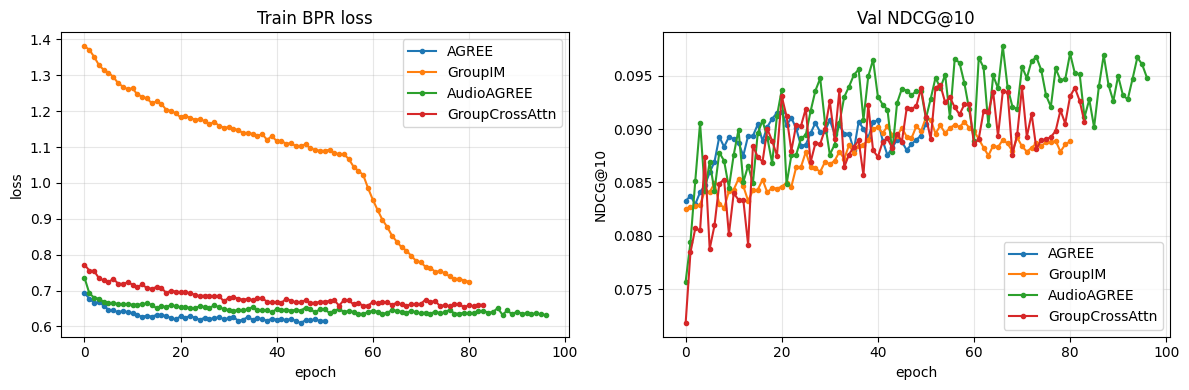
\includegraphics[width=0.95\textwidth]{graphics/train_4_approaches.png}
    \caption{Кривые обучения четырёх агрегаторов: train loss и val~NDCG@10 по эпохам. Audio-методы (Audio-AGREE, Group Cross-Attention) выходят на более высокий уровень val-метрики относительно ID-методов (AGREE, GroupIM).}
    \label{fig:train-4-approaches}
\end{figure}

\subsection{Оценка и статистический протокол}\label{subsec:ch3:eval-protocol}

\paragraph{Метрики.} В качестве основной метрики используется групповой $\mathrm{NDCG@K}$, $K \in \{10, 20\}$:
\begin{equation}
    \mathrm{NDCG@K}(G) = \frac{1}{\mathrm{IDCG@K}(G)} \sum_{k=1}^{K} \frac{\mathbf{1}[i_k \in \mathcal{Y}_G^{\mathrm{test}}]}{\log_2(k + 1)},
\end{equation}
где $i_k$~--- $k$-й трек ранжированного списка $\mathrm{Rec}_K(G) = \mathrm{argtop}\text{-}K_{i \in \mathcal{C}_G}\, \hat{s}_{G, i}$, а $\mathrm{IDCG@K}(G)$~--- значение DCG@K при идеальном ранжировании внутри $\mathcal{C}_G$. Усреднение по группам производится после фильтрации групп с пустым $\mathcal{Y}_G^{\mathrm{test}}$.

Метрики справедливости и разнообразия (Jain@K, Disagreement@K, сводная DFH@K)~--- стандартные для литературы по групповым рекомендациям~\cite{jin2023fairness_survey}~--- сформулированы методически и обсуждаются в разделе~\ref{sec:ch3:limitations} как направление развития. Их вычисление на готовом per-sample наборе скоров $\{\hat{s}_{G, i}\}_{G, i}$ тривиально и не требует переобучения моделей.

\paragraph{Бутстрап доверительные интервалы.} Для каждого метода NDCG-метрика и её 95\%-CI рассчитываются бутстрапом по группам с числом репликаций $N_{\mathrm{boot}} = 1{,}000$. Принципиальное методологическое решение~--- \emph{единая resample-сетка для всех методов}: один и тот же массив индексов $\mathtt{resample\_idx}[N_{\mathrm{boot}}, n_{\mathrm{groups}}]$, сгенерированный фиксированным сидом ($\mathtt{seed} = 42$), используется при подсчёте маргинальных CI для каждого из семи методов. Это даёт два эффекта: (а) маргинальные CI согласованы между собой~--- разница средних между методами автоматически совпадает с paired-разностью на той же выборке; (б) paired-bootstrap для попарных сравнений переиспользует ту же сетку, что обеспечивает идентичный шум выборки в маргинальной и paired-статистике.

\paragraph{Paired bootstrap (audio − ID).} Для центральной гипотезы H1 (audio $>$ ID) репортируется paired-bootstrap-разность $\Delta_{\mathrm{audio} - \mathrm{ID}}^{(b)} = \overline{\mathrm{NDCG}}_{\mathrm{audio}}^{(b)} - \overline{\mathrm{NDCG}}_{\mathrm{ID}}^{(b)}$ для каждой репликации $b = 1, \ldots, N_{\mathrm{boot}}$. 95\%-CI разности~--- эмпирические перцентили распределения $\{\Delta_{\mathrm{audio} - \mathrm{ID}}^{(b)}\}_{b}$. Одностороннее $p$-значение~--- доля репликаций, на которых $\Delta_{\mathrm{audio} - \mathrm{ID}}^{(b)} \leq 0$. Сравниваются четыре пары audio${\times}$ID: $\{\text{Audio-AGREE}, \text{Group Cross-Attention}\} \times \{\text{AGREE}, \text{GroupIM}\}$, при $K \in \{10, 20\}$~--- всего 8 paired-сравнений. All-pairs-сравнение (включая audio${\times}$audio и ID${\times}$ID) намеренно не строится: гипотеза H1 минимальная и формулирует только противопоставление audio vs ID; расширение на all-pairs увеличило бы шум на коррекции множественных сравнений без содержательной отдачи.

\paragraph{Обоснование выбора paired bootstrap.} Альтернативные статистические подходы~--- классический $t$-тест на средних, Wilcoxon signed-rank на per-sample-разностях, permutation-test~--- в принципе применимы и часто используются в литературе по рекомендательным системам. Выбор paired-bootstrap обоснован тремя соображениями. Во-первых, бутстрап-CI на per-group-разностях $\Delta_G = \mathrm{NDCG}_{\mathrm{audio}}(G) - \mathrm{NDCG}_{\mathrm{ID}}(G)$ не требует предположения о нормальности или симметрии распределения разностей, что в условиях смешанного распределения групп по размеру и составу более защищено. Во-вторых, общая resample-сетка обеспечивает согласованность маргинальных и paired-статистик~--- свойство, которое $t$-тест и Wilcoxon не дают <<из коробки>>. В-третьих, paired-bootstrap даёт распределение разностей, из которого тривиально извлекается как CI, так и $p$-значение, что упрощает интерпретацию.

\paragraph{Срез по размеру группы.} В дополнение к общему сравнению NDCG-метрика рассчитывается отдельно для каждого размера группы $|G| \in \{2, 3, 4, 5\}$~--- четыре независимые resample-сетки, $N_{\mathrm{boot}} = 1{,}000$ каждая. Это даёт количественную оценку того, как преимущество audio-методов зависит от $|G|$~--- ожидаемое теоретическое следствие из того, что при росте $|G|$ возрастает разнообразие вкусов внутри группы, и item-aware attention поверх содержательного сигнала (аудио) должен иметь больше пространства для дифференциации членов, чем поверх ID-эмбеддингов.

\section{Результаты}\label{sec:ch3:results}

\subsection{Сводная таблица}\label{subsec:ch3:results-table}

Финальная сводная таблица сравнения семи методов по NDCG@10 и NDCG@20 на тестовой выборке из 2{,}000 синтетических случайных групп приведена в таблице~\ref{tab:results-main}. Все значения сопровождаются 95\%-бутстрап-CI, рассчитанными по общей resample-сетке.

\begin{table}[ht]
    \centering
    \caption{Сравнение групповых агрегаторов на тесте (2{,}000 случайных групп, размер 2--5, $N_{\mathrm{boot}} = 1{,}000$). Жирным выделены два лучших метода. Audio-методы превосходят все остальные на обоих $K$.}
    \label{tab:results-main}
    \small
\begin{tabular}{lcc}
    \toprule
    Метод & NDCG@10 (95\% CI) & NDCG@20 (95\% CI) \\
    \midrule
    Group Cross-Attn & $\mathbf{0{,}0916}$ [$0{,}0830$; $0{,}1002$] & $\mathbf{0{,}0958}$ [$0{,}0873$; $0{,}1042$] \\
    Audio-AGREE      & $\mathbf{0{,}0901}$ [$0{,}0823$; $0{,}0990$] & $\mathbf{0{,}0947}$ [$0{,}0862$; $0{,}1030$] \\
    MP               & $0{,}0828$ [$0{,}0751$; $0{,}0906$] & $0{,}0859$ [$0{,}0782$; $0{,}0937$] \\
    GroupIM          & $0{,}0811$ [$0{,}0735$; $0{,}0887$] & $0{,}0846$ [$0{,}0770$; $0{,}0922$] \\
    AGREE            & $0{,}0790$ [$0{,}0718$; $0{,}0860$] & $0{,}0835$ [$0{,}0763$; $0{,}0907$] \\
    AVG              & $0{,}0712$ [$0{,}0645$; $0{,}0781$] & $0{,}0748$ [$0{,}0680$; $0{,}0816$] \\
    LM               & $0{,}0312$ [$0{,}0268$; $0{,}0357$] & $0{,}0361$ [$0{,}0314$; $0{,}0408$] \\
    \bottomrule
\end{tabular}
\end{table}

\paragraph{Ключевые наблюдения.} Из таблицы~\ref{tab:results-main} следуют четыре содержательных вывода, развёрнуто обсуждаемых ниже.
\begin{enumerate}
    \item Оба audio-метода (Group Cross-Attention, Audio-AGREE) занимают первые две позиции по обеим метрикам.
    \item Тривиальная стратегия MP опережает оба обучаемых ID-метода (AGREE, GroupIM)~--- сильный аргумент о структурном пределе ID-сигнала поверх замороженного скорера.
    \item Маргинальные CI пар <<лучший audio>> и <<MP>> существенно перекрываются, что на первый взгляд ставит под сомнение значимость преимущества audio-методов. Paired bootstrap (подраздел~\ref{subsec:ch3:paired}) показывает, что это перекрытие~--- эффект совместного шума, а не отсутствия эффекта.
    \item LM (Least Misery) демонстрирует выраженный провал ($\mathrm{NDCG@10} = 0{,}031$), почти втрое уступая AVG. Причина обсуждается в подразделе~\ref{subsec:ch3:results-discuss}.
\end{enumerate}

\subsection{Paired bootstrap: значимость преимущества audio над ID}\label{subsec:ch3:paired}

Маргинальные 95\%-CI пар <<Audio-AGREE / Group Cross-Attention>> и <<AGREE / GroupIM>> в таблице~\ref{tab:results-main} существенно перекрываются (например, для $K = 10$: $[0{,}0823, 0{,}0990]$ у Audio-AGREE и $[0{,}0718, 0{,}0860]$ у AGREE). Если интерпретировать перекрытие CI как отсутствие значимого различия, то гипотеза H1 не подтверждается~--- но такая интерпретация некорректна. Маргинальные CI рассчитываются по неcoupled-распределениям и игнорируют корреляцию между методами через общие группы: одна и та же <<сложная>> группа $G$ занижает NDCG у всех методов одновременно, и часть наблюдаемой маргинальной дисперсии~--- общая.

Paired bootstrap исключает эту общую часть, рассчитывая распределение per-group-разностей $\{\Delta_G\}_{G}$ напрямую. Результаты восьми парных сравнений приведены в таблице~\ref{tab:paired}.

\begin{table}[ht]
    \centering
    \caption{Paired bootstrap audio vs ID. Положительное $\Delta$~--- audio-метод лучше ID-метода. CI и $p$-значение по 1{,}000 репликаций на общей resample-сетке.}
    \label{tab:paired}
    \begin{tabular}{llccc}
        \toprule
        Audio & ID & $K$ & $\Delta$ mean (95\% CI) & $p$ one-sided \\
        \midrule
        Audio-AGREE & AGREE & 10 & $+0{,}0110\ [0{,}0053,\ 0{,}0177]$ & $<0{,}001$ \\
        Audio-AGREE & AGREE & 20 & $+0{,}0112\ [0{,}0052,\ 0{,}0176]$ & $<0{,}001$ \\
        Audio-AGREE & GroupIM & 10 & $+0{,}0090\ [0{,}0024,\ 0{,}0154]$ & $0{,}005$ \\
        Audio-AGREE & GroupIM & 20 & $+0{,}0101\ [0{,}0037,\ 0{,}0164]$ & $0{,}001$ \\
        GroupCrossAttn & AGREE & 10 & $+0{,}0125\ [0{,}0054,\ 0{,}0194]$ & $<0{,}001$ \\
        GroupCrossAttn & AGREE & 20 & $+0{,}0123\ [0{,}0059,\ 0{,}0190]$ & $<0{,}001$ \\
        GroupCrossAttn & GroupIM & 10 & $+0{,}0105\ [0{,}0033,\ 0{,}0175]$ & $0{,}001$ \\
        GroupCrossAttn & GroupIM & 20 & $+0{,}0112\ [0{,}0046,\ 0{,}0178]$ & $<0{,}001$ \\
        \bottomrule
    \end{tabular}
\end{table}

Во всех восьми сравнениях 95\%-CI разности не пересекает~0 и одностороннее $p$-значение $\leq 0{,}005$. Гипотеза~H1 подтверждается на тесте по всем четырём audio${\times}$ID-парам и обоим $K$. Абсолютное преимущество audio-методов составляет $\Delta \in [0{,}009, 0{,}013]$ по NDCG@10/20, что в относительных терминах~--- $\sim 12$--$16\%$ от уровня ID-методов. Визуализация рассмотренных пар в форме forest plot приведена на рис.~\ref{fig:forest-plot}.

\begin{figure}[ht]
    \centering
    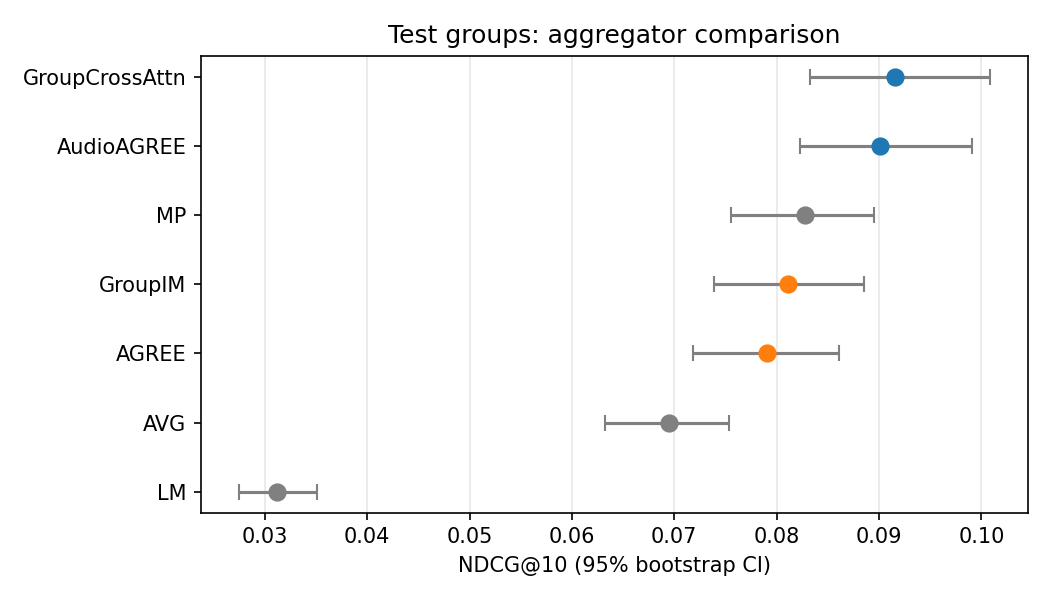
\includegraphics[width=0.95\textwidth]{graphics/eval_forest_plot.png}
    \caption{Forest plot paired-разностей audio−ID и маргинальных значений NDCG@10/20 для семи методов. Все восемь paired-разностей значимо положительны (CI не пересекает~0).}
    \label{fig:forest-plot}
\end{figure}

\subsection{Срез по размеру группы}\label{subsec:ch3:results-size}

Зависимость NDCG@10 от размера группы $|G| \in \{2, 3, 4, 5\}$ для всех семи методов приведена в таблице~\ref{tab:results-by-size} и визуализирована на рис.~\ref{fig:ndcg-by-size}~и~\ref{fig:heatmap-method-size}.

\begin{table}[ht]
    \centering
    \caption{NDCG@10 по размеру группы. Жирным выделены лучшие методы в каждом столбце.}
    \label{tab:results-by-size}
    \begin{tabular}{lcccc}
        \toprule
        Метод & $|G|=2$ & $|G|=3$ & $|G|=4$ & $|G|=5$ \\
        \midrule
        AGREE             & $0{,}095$ & $0{,}073$ & $0{,}073$ & $0{,}078$ \\
        GroupIM           & $0{,}104$ & $0{,}072$ & $0{,}074$ & $0{,}077$ \\
        Audio-AGREE       & $0{,}110$ & $0{,}078$ & $\mathbf{0{,}090}$ & $\mathbf{0{,}089}$ \\
        Group Cross-Attn  & $\mathbf{0{,}115}$ & $\mathbf{0{,}081}$ & $0{,}087$ & $\mathbf{0{,}089}$ \\
        MP                & $0{,}105$ & $0{,}076$ & $0{,}076$ & $0{,}072$ \\
        AVG               & $0{,}094$ & $0{,}065$ & $0{,}057$ & $0{,}056$ \\
        LM                & $0{,}044$ & $0{,}027$ & $0{,}027$ & $0{,}028$ \\
        \bottomrule
    \end{tabular}
\end{table}

\begin{figure}[ht]
    \centering
    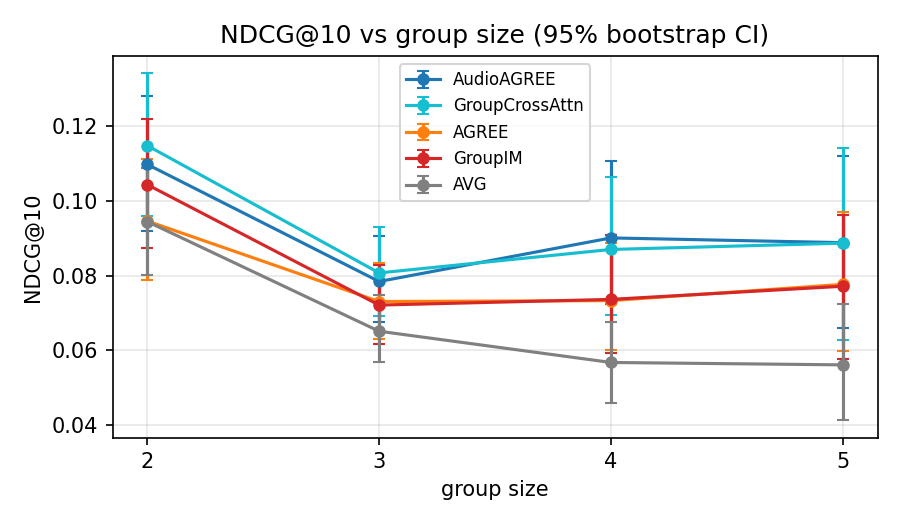
\includegraphics[width=0.85\textwidth]{graphics/eval_ndcg_by_size.png}
    \caption{NDCG@10 в зависимости от размера группы. Audio-методы устойчиво лидируют на $|G| \geq 3$; на $|G| = 2$ преимущество не выражено.}
    \label{fig:ndcg-by-size}
\end{figure}

\begin{figure}[ht]
    \centering
    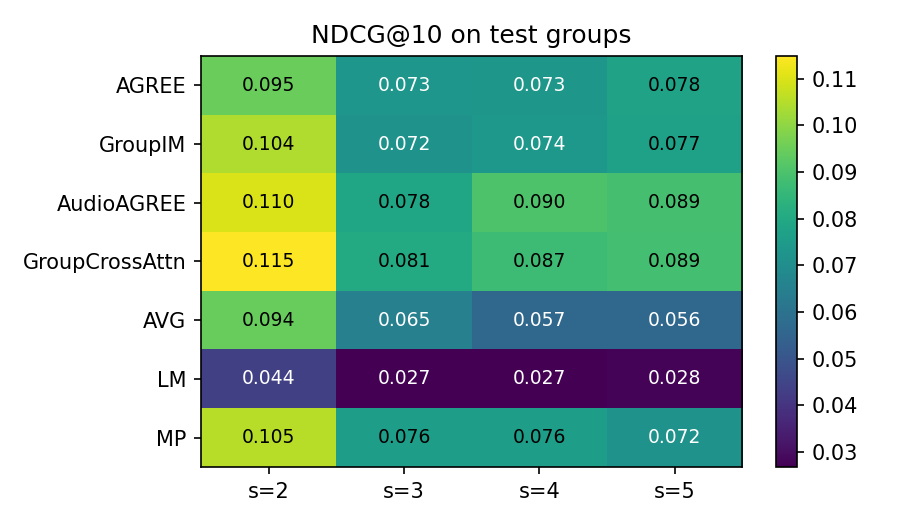
\includegraphics[width=0.85\textwidth]{graphics/eval_heatmap_method_size.png}
    \caption{Heatmap метод${\times}$размер группы по NDCG@10. Тёмный край у audio-методов на $|G| \in \{4, 5\}$ показывает источник их общего преимущества~--- группы среднего размера.}
    \label{fig:heatmap-method-size}
\end{figure}

\paragraph{Качественный паттерн.} На парных группах ($|G| = 2$) все обучаемые методы и MP плотно сбиты в диапазон $0{,}095$--$0{,}115$, а тривиальные AVG/LM отстают. На группах большего размера ($|G| \in \{3, 4, 5\}$) ID-методы и MP стагнируют на уровне $\sim 0{,}072$--$0{,}077$, AVG проседает до $0{,}056$--$0{,}065$, а audio-методы держат $0{,}078$--$0{,}090$. Относительный gap audio vs лучший-из-не-audio при $|G| = 4$ составляет $+18\%$ (Audio-AGREE $0{,}090$ vs MP $0{,}076$), при $|G| = 5$~--- $+17\%$ (Audio-AGREE/Group Cross-Attention $0{,}089$ vs AGREE $0{,}078$).

Этот паттерн содержательно интерпретируется. На парных группах задача агрегации структурно проще: множество $\{\hat{s}_{u, i}\}_{u \in G}$ состоит из двух чисел, и почти любая монотонная агрегация даёт близкий результат. На больших группах вклад каждого члена становится более <<разреженным>>, и качество агрегации определяется тем, насколько модель умеет различать членов группы между собой~--- то есть качеством используемого attention-сигнала. Аудиоэмбеддинги, дающие непрерывный content-based сигнал, превосходят обучаемые ID-эмбеддинги в этой роли при фиксированном скорере и ограниченном объёме обучающих данных.

\subsection{Обсуждение}\label{subsec:ch3:results-discuss}

\paragraph{Audio значимо обходит ID.} Гипотеза H1 подтверждается на тесте. Абсолютный gap $\Delta \approx +0{,}011$ по NDCG@10/20 невелик в маргинальных терминах, но устойчиво обнаруживается paired-bootstrap'ом с $p \leq 0{,}005$ и не пересекает~0 ни в одной из восьми проверенных пар. Это критичная для интерпретации деталь: маргинальные CI создают впечатление, что эффект на грани шума~--- на самом деле эффект устойчив, а большая часть маргинальной дисперсии~--- общий шум выборки групп, разделяемый всеми методами.

\paragraph{MP $>$ обучаемые ID-методы.} Тривиальный максимум по членам группы (MP) опережает оба обучаемых ID-метода в общей таблице ($0{,}0828 > 0{,}0811 > 0{,}0790$). Этот результат~--- сильный аргумент в пользу того, что \emph{обучаемые ID-attention поверх замороженного SASRec не дают полезного сигнала сверх тривиального максимума}. Возможные объяснения: (а)~item-эмбеддинги AGREE/GroupIM не имеют доступа к семантике треков и обучаются только на синтетических группах, что недостаточно для содержательного сигнала; (б)~замороженный SASRec уже выдаёт хорошо откалиброванные персональные скоры~--- максимум по членам естественно выделяет <<наиболее увлечённого>> кандидата, и обучаемая агрегация поверх лишь добавляет шум. Аудио-сигнал, в отличие от ID, доступен напрямую и не требует обучения~--- это и позволяет ему пробить структурный потолок.

\paragraph{Два audio-варианта статистически неразличимы.} Маргинальные CI Audio-AGREE ($0{,}0901$) и Group Cross-Attention ($0{,}0916$) полностью перекрываются; на val (по результатам обучения) порядок был обратный. Формулировка для содержательного вывода: выбор между однопроекционным MLP-attention и многоголовым dot-product не критичен~--- важен сам факт использования аудиосигнала. С позиции инженерной простоты Audio-AGREE предпочтительнее (один MLP против $2H$ линейных проекций), с позиции теоретической согласованности с трансформерной литературой~--- Group Cross-Attention. Для задач, в которых $d_a$ больше нашего ($128$) или ожидается высокая структурная неоднородность кандидатов, многоголовое attention~--- более защищённая ставка.

\paragraph{Провал LM.} Least Misery (минимум по членам группы) даёт NDCG@10 = $0{,}0312$~--- втрое ниже AVG. Причина связана с устройством $\mathtt{fill} = 0$ для item $\notin \mathrm{top}\text{-}K_{\mathrm{cache}}(u)$ и фактическим диапазоном скоров $[-0{,}22, 17{,}26]$. Любой трек, не входящий в топ-200 хотя бы одного члена группы, получает $\min = 0$ от LM; реально хорошие кандидаты, попавшие в топ-200 \emph{не у всех} членов, при этом тоже занижаются. AVG, напротив, усредняет ненулевой вклад тех членов, у кого трек попал в топ, что даёт более устойчивое ранжирование. LM в таблице играет роль negative control, оправдывающего выбор AVG и MP как <<настоящих>> тривиалов.

\paragraph{Структурное плато.} Совпадение метрик AGREE и GroupIM до четвёртого знака (val~$0{,}091$ vs $0{,}091$ на эпохе остановки) и независимость от продления обучения с 60 до 100 эпох~--- свидетельство достижения структурного предела ID-сигнала поверх замороженного скорера. Аналитически: BPR-loss упирается в потолок, заданный фиксированными $\hat{s}_{u, i}$~--- максимум различимости между группами определяется тем, насколько per-user-скоры уже разделяют членов одной группы, а агрегатор может лишь перевзвесить уже имеющийся сигнал. Audio-сигнал даёт независимый источник информации (через $\bar{\mathbf{a}}_u$ и $\mathbf{a}_i$) и потому пробивает потолок; ID-сигнал, который ничем не подкреплён извне, потолок воспроизвести не может. Это~--- центральное методологическое наблюдение работы.

\section{Вычислительные ресурсы и воспроизводимость}\label{sec:ch3:compute}

Полный объём YAMBDA-500m ($4{,}79 \cdot 10^9$ событий) превышает доступные вычислительные ресурсы на несколько порядков. Все эксперименты выполнены в условиях ограниченного облачного бюджета, что определяет ряд практических решений и одновременно задаёт рамку для воспроизводимости.

\subsection{Среда выполнения}\label{subsec:ch3:compute-env}

Используются два класса GPU-сред Google Colab и одна локальная машина.

\textbf{Колаб A100 (40~ГБ HBM, 80~ГБ RAM)} применяется в Phase~1 для обучения per-user скорера на полной фильтрованной выборке YAMBDA-50m. Полный цикл воспроизведения яндексовского baseline (раздел~\ref{subsec:ch3:setup-gap})~--- порядка $10$ часов чистого времени GPU с учётом всех итераций по конфигу.

\textbf{Колаб G4 (NVIDIA L4, $\sim$95~ГБ RAM)} применяется в Phase~2 для обучения и оценки групповых агрегаторов. Больший объём оперативной памяти позволяет держать subset аудиоэмбеддингов ($135$~МБ) целиком in-memory и убирает необходимость в \texttt{memmap}-доступе. Прогон всех четырёх обучаемых агрегаторов (раздел~\ref{subsec:ch3:aggregators}) занимает менее $10$ минут; полная оценка с paired-bootstrap'ом~--- порядка $2$ минут.

\textbf{Локальная машина (MacBook Pro M4~Pro, 24~ГБ unified memory)} используется как smoke-среда: проверка корректности кода на малых батчах перед запуском на Colab, разведочный анализ данных, генерация графиков, сборка LaTeX. Все нейросетевые обучения вынесены в облако~--- локальный CPU/GPU не задействуется.

В качестве программного стека используются \texttt{Python~3.11}, \texttt{PyTorch} (нейросетевые модели и обучение), \texttt{NumPy}, \texttt{pandas}, \texttt{Polars} (предварительная обработка), \texttt{pyarrow} (range-read parquet с HuggingFace Hub), \texttt{scikit-learn} и \texttt{SciPy} (вспомогательные статистики), \texttt{matplotlib} (графики). Полный список зависимостей с фиксированными версиями приведён в \texttt{requirements.txt} в корне репозитория работы.

\subsection{Управление вычислительной стоимостью}\label{subsec:ch3:compute-cost}

Главным compute-trick'ом, делающим возможным многократный запуск групповых экспериментов на одном-двух часах G4, является \emph{кэширование скоров замороженного скорера}.

\textbf{Кэш per-user топ-$K$.} Выход обученного SASRec~--- топ-$200$ персональных скоров на каждого пользователя (раздел~\ref{subsec:ch3:cache})~--- вычисляется однократно после фиксации скорера и сохраняется как parquet-файл размером $1{,}83$~млн строк. Все последующие эксперименты с групповыми агрегаторами читают этот кэш как табличный артефакт и не запускают нейросетевую модель ни на одном батче. Это сокращает время цикла «правка кода~$\to$ повтор эксперимента» с десятков минут до секунд и позволяет проводить попарные сравнения четырёх агрегаторов на едином compute-бюджете.

\textbf{Range-read аудиоэмбеддингов.} Полный файл аудиоэмбеддингов YAMBDA весит $14$~ГБ ($7{,}72$~млн треков $\times$ $128$). Скачивание целиком на Colab-диск нерационально; вместо этого используется потоковое чтение через \texttt{HfFileSystem}: parquet-файл открывается удалённо, в память поднимаются только две колонки (\texttt{item\_id}, \texttt{embedding}), затем выполняется фильтрация по $276\,305$ item\_id из Phase~1. Результирующий subset ($\sim$$135$~МБ, float32) сохраняется на диск как \texttt{embeddings.npy} и более не пересчитывается. Этот приём описан подробно в разделе~\ref{subsec:ch3:audio}; здесь он фигурирует как ключевой элемент compute-плана.

\textbf{Усечение пространства кандидатов.} На уровне группы пул $\mathcal{C}_G = \bigcup_{u \in G} \mathrm{top}\text{-}K_{\mathrm{cache}}(u)$ ограничивает оценку $|G| \times \sim$$200$ позициями вместо полного каталога $276{\rm k}$ items, что делает один проход агрегатора по batch\textsubscript{64} вопросом миллисекунд.

\textbf{Разделение «код~/~артефакты».} Исходный код версионируется в git, тяжёлые артефакты (чекпоинт SASRec, кэш скоров, subset аудиоэмбеддингов, чекпоинты агрегаторов, eval-таблицы) хранятся в HuggingFace-репозитории \texttt{Vladislavbro-500/music-recommendations} (тип \emph{dataset}) и подтягиваются на Colab идемпотентным \texttt{hf\_hub\_download} с пропуском уже скачанных файлов. Такая разводка соответствует стандартному паттерну для Colab-экспериментов и одновременно обеспечивает атомарную публикацию артефактов под фиксированной версией кода.

\subsection{Воспроизводимость}\label{subsec:ch3:reproducibility}

Воспроизводимость обеспечивается на нескольких уровнях.

\textbf{Фиксация случайных операций.} Все случайные генераторы~--- \texttt{Python random}, \texttt{NumPy}, \texttt{PyTorch} (CPU и CUDA)~--- инициализируются единым сидом через хелпер \texttt{src/utils/seed.py::set\_seed}. При \texttt{deterministic\_torch=True} дополнительно включается детерминированный режим \texttt{cuDNN} с отключённым автотюнером. Сид per-user обучения~--- $42$; сид синтеза групп~--- $42$; сид bootstrap-resampling'а~--- $42$. Совпадение сидов между этапами не критично (этапы независимы), но эксплицитно зафиксировано для прозрачности.

\textbf{Версионирование экспериментальных артефактов.} Сплиты пользователей и треков, отображение \texttt{item\_id\_to\_idx}, фиксированный split групп \texttt{groups\_split.pkl} (состав \texttt{train\_groups}, \texttt{val\_groups}, \texttt{test\_groups} + \texttt{group\_seed}, \texttt{size\_dist}, статистика по targets) сохраняются вместе с кодом и обеспечивают побитовую идентичность данных между запусками. Тестовые группы синтезируются однократно на этапе обучения агрегаторов и не меняются на этапе финальной оценки~--- это исключает возможность непреднамеренной подгонки под test.

\textbf{Бутстрап с сохранением resample-индексов.} Файл \texttt{per\_sample.npz} содержит не только пер-семпловые значения NDCG@10/20 для каждого метода, но и саму матрицу resample-индексов \texttt{resample\_idx} формы $[B, n]$, \texttt{int32}, где $B = 1000$, $n$~--- число test-групп. Любой третий сторонний наблюдатель, имея эту матрицу, может воспроизвести любое CI и любой paired-test из таблицы~\ref{tab:paired-bootstrap} без обращения к ГПСЧ.

\textbf{Конфиги рядом с чекпоинтами.} Для каждой обученной модели (один скорер + четыре агрегатора) рядом с весами лежит \texttt{config.json} с полным набором гиперпараметров, использованных при обучении, и \texttt{metrics.csv} с историей train/val метрик. Это позволяет восстановить точную постановку каждого эксперимента без обращения к коду.

\textbf{Публикация кода и артефактов.} Исходный код, конфигурации, ноутбуки и журналы экспериментов опубликованы в открытом репозитории; артефакты~--- в открытом HuggingFace-репозитории. Совокупность \texttt{git-commit-hash} + \texttt{HF-revision-hash} однозначно фиксирует версию эксперимента.

\section{Ограничения исследования и направления развития}\label{sec:ch3:limitations}

Настоящий раздел организован как карта развития. Каждое направление сопровождается (а)~описанием ограничения и его влияния на текущие результаты, (б)~указанием на компенсирующий приём (если он применён в работе), (в)~эскизом расширения, которое естественно ляжет в основу журнальной статьи на материале диссертации. Изложение разделено на четыре блока: методологические ограничения двухуровневой рамки, расширение протокола оценки, расширение методологии экспериментов, расширение методики.

\subsection{Методологические ограничения и их компенсация}\label{subsec:ch3:lim-methodology}

\textbf{Замороженный скорер vs совместное обучение.} Главное архитектурное решение работы~--- фиксация per-user скорера и обучение только агрегатора~--- по дизайну (раздел~\ref{subsec:ch3:framework}) обеспечивает чистую ablation вклада агрегационного механизма и согласован с индустриальной two-stage retrieval-rerank рамкой. Это же решение ограничивает обнаруживаемый эффект потолком, заданным фиксированными $\hat{s}_{u, i}$: разделимость членов одной группы по персональным скорам определяется качеством скорера, а агрегатор может лишь перевзвесить уже имеющийся сигнал. Эмпирически этот потолок виден в структурном плато ID-методов (раздел~\ref{subsec:ch3:results-discuss}). Естественное расширение~--- сценарий с лёгким end-to-end fine-tune скорера под группой BPR-loss: два parameter group в Adam (\texttt{lr}\textsubscript{aggregator}~$=10^{-3}$, \texttt{lr}\textsubscript{scorer}~$=10^{-5}$), knowledge-distillation регуляризация на solo-user тесте против catastrophic forgetting и сопоставление с замороженной рамкой по той же метрической сетке. Этот сценарий оформляется как самостоятельная гипотеза H2 в будущей статье~--- «End-to-end совместное обучение скорера и агрегатора расширяет gap audio~$>$~ID за счёт обновления per-user-сигнала под групповую задачу»~--- и не подменяет нынешний результат, а дополняет его.

\textbf{Объём обучения и статистическая мощность.} После канонической фильтрации YAMBDA-50m остаётся $9{,}2$~тыс. пользователей и $276$~тыс. треков (раздел~\ref{sec:ch3:data})~--- порядок, типичный для академических групповых работ, но являющийся нижней границей для тонких эффектов. В работе это компенсировано (а)~paired-bootstrap'ом на общей resample-сетке (раздел~\ref{subsec:ch3:eval-protocol}), который обеспечивает стат. уверенность при умеренном $n$, и (б)~вынесением сравнения архитектурных вариантов audio-aware агрегатора в обсуждение «статистически неразличимы», а не в самостоятельный результат. Прямое расширение~--- переход на YAMBDA-500m: общее количество users увеличивается на порядок (по аннотации датасета~\cite{yambda2025}), что позволит надёжно различить тонкие архитектурные эффекты внутри audio-семейства и провести замеры на гетерогенных подвыборках с меньшей дисперсией.

\textbf{Только random-группы.} Все обучение и финальная оценка проведены на random-группах из обучающего временного окна. Это сознательное методологическое решение: совпадение распределений обучения и оценки по характеристикам сходства членов привело бы к ситуации, в которой выигрыш модели объяснялся бы подгонкой под распределение, а не качеством агрегационного механизма. Развитие~--- срез по гомогенности группы (см. подраздел~\ref{subsec:ch3:lim-eval-protocol}).

\subsection{Развитие протокола оценки}\label{subsec:ch3:lim-eval-protocol}

В основной таблице сравнения зарепортированы только NDCG@10/20 (раздел~\ref{subsec:ch3:results-table}). Это сознательное упрощение под фиксированный compute-бюджет и доступный объём данных; ниже перечислены направления расширения метрической сетки, методически проработанные на этапе планирования и оставленные для будущей статьи.

\textbf{Метрики справедливости и разнообразия.} \emph{Jain@K} как нормированный в $[0, 1]$ индекс Джейна устойчив к нулевым значениям~\cite{jin2023fairness_survey} и измеряет равномерность удовлетворённости членов группы:
\begin{equation}
    \mathrm{Jain}(G, K) = \frac{ \left( \sum_{u \in G} \mathrm{Sat}_u(G, K) \right)^2 }{ |G| \cdot \sum_{u \in G} \mathrm{Sat}_u(G, K)^2 },
    \label{eq:jain}
\end{equation}
где $\mathrm{Sat}_u(G, K)$~--- индивидуальная удовлетворённость члена $u$ итоговым списком группы (например, его персональный NDCG@K по списку $\mathrm{Rec}_K(G)$). Значение $1$ соответствует абсолютно равномерной удовлетворённости, $1/|G|$~--- режиму «удовлетворён ровно один». \emph{Disagreement@K} как стандартное отклонение $\{\mathrm{Sat}_u(G, K)\}_{u \in G}$ дополняет Jain симметричной мерой разноса. \emph{DFH@K} как гармоническое среднее качества и справедливости даёт сводный показатель:
\begin{equation}
    \mathrm{DFH@K}(G) = \frac{2 \cdot \mathrm{NDCG@K}(G) \cdot \mathrm{Jain}(G, K)}{ \mathrm{NDCG@K}(G) + \mathrm{Jain}(G, K) }.
    \label{eq:dfh}
\end{equation}
В журнальной постановке предполагается раздельный репорт NDCG@K и Jain@K с приоритетом интерпретации, и DFH@K как вспомогательный композитный критерий выбора гиперпараметров на валидации. Использование гармонического среднего величин разного масштаба (типичный NDCG@K в диапазоне $0{,}05$--$0{,}25$ против Jain@K $0{,}6$--$1{,}0$) методологически нетривиально и требует отдельной оговорки в тексте.

\textbf{Cold-start срез.} Подвыборка $\mathcal{I}_{\mathrm{cold}} = \{i \in \mathcal{I} : \mathrm{count}_{\mathrm{train}}(i) \leq n_{\mathrm{cold}}\}$ при фиксированном пороге $n_{\mathrm{cold}}$ (предполагаемое значение даёт $|\mathcal{I}_{\mathrm{cold}}| / |\mathcal{I}| \sim 10$--$20\%$) и переопределение релевантных множеств $\mathcal{R}_u^{\mathrm{cold}} = \mathcal{R}_u \cap \mathcal{I}_{\mathrm{cold}}$ позволяют количественно оценить, насколько преимущество audio-aware агрегатора связано именно со способностью работать на редких треках. Гипотеза для статьи~--- «gap audio~$>$~ID растёт с долей редких треков в кандидатном пуле» (содержательно обоснована тем, что ID-эмбеддинги обучаемых агрегаторов не имеют доступа к семантике треков, тогда как $\mathbf{a}_i$ доступен для любого трека из каталога независимо от его частоты).

\textbf{Гомогенные и гетерогенные группы.} В качестве меры сходства предлагается коэффициент Жаккара по множествам прослушанных треков $\mathrm{sim}(u, v) = |\mathcal{S}_u \cap \mathcal{S}_v| / |\mathcal{S}_u \cup \mathcal{S}_v|$~--- сознательно не аудио-косинус, чтобы исключить циркулярность с предлагаемым агрегатором. Гомогенные группы формируются из пар $(u, v)$ с $\mathrm{sim}(u, v) \geq \tau_{\mathrm{hom}}$, гетерогенные~--- с $\mathrm{sim}(u, v) \leq \tau_{\mathrm{het}}$. Ожидаемая интерпретация: audio-aware агрегатор сильнее выигрывает на гетерогенных группах, где разделимость членов по содержательному сигналу содержательно важнее.

\subsection{Развитие методологии экспериментов}\label{subsec:ch3:lim-methodology-eval}

\textbf{Replication runs в дополнение к bootstrap.} В работе зафиксирован один обучающий run на конфиг (с единым seed); статистическая уверенность обеспечивается paired-bootstrap'ом по test-группам. Это~--- осознанный размен compute-бюджета на статистическую глубину анализа. Расширение~--- $n_{\mathrm{seeds}} = 5$ запусков с разными random-сидами для каждой архитектуры. Это позволит разделить два источника дисперсии: (а)~дисперсию выборки групп (текущий bootstrap), (б)~дисперсию инициализации и порядка обучающих батчей (текущая работа этот источник не покрывает). При $n_{\mathrm{seeds}} = 5$ репортируется среднее $\pm$~std по сидам в сочетании с paired-bootstrap CI; гипотеза H1 на этих данных проверяется иерархическим бутстрапом по группам и сидам.

\textbf{Sweep гиперпараметров в едином compute-бюджете.} Для основной таблицы использовалась одна конфигурация на метод (single config per method), что согласуется с дефолтами AGREE / GroupIM и обеспечивает honest сравнение четырёх обучаемых агрегаторов при одинаковом compute-бюджете. Тонкие гиперпараметры~--- $\lambda_{\mathrm{MI}}$ для GroupIM, $d_{\mathrm{att}}$ и $d_{\mathrm{model}}$ для audio-методов, $H$ для Group Cross-Attention~--- зафиксированы по дефолтам. Расширение~--- случайный sweep ($\sim$$30$--$50$ конфигов на метод) с фиксированным total-compute-budget и выбором лучшего по val~NDCG@10. Особый интерес~--- $\lambda_{\mathrm{MI}} \in \{0{,}1,\ 0{,}5,\ 1{,}0\}$ для GroupIM (используется значение $0{,}5$ как середина паперной сетки; sweep отложен) и сравнение bilinear-дискриминатора MI с MLP-альтернативой.

\textbf{Поведенческая валидация аудиоэмбеддингов.} Аудиоэмбеддинги YAMBDA предоставляются без открытой документации обучающей процедуры и без открытых семантических зондов (тип жанра, темп, тональность). В работе они приняты как чёрный ящик и подвергнуты только эмпирической проверке через performance в рекомендационной задаче. Расширение~--- три поведенческих зонда: (а)~ко-встречаемость близких эмбеддингов в одной сессии слушания (вес ребра графа cos-similarity vs частота совместного появления; ожидаемая корреляция $\rho > 0{,}5$), (б)~кластеризация $k$-means по эмбеддингам и сравнение кластеров с track-id-based ко-встречаемостью (mutual information), (в)~стабильность пользовательского профиля $\bar{\mathbf{a}}_u$ во времени (косинус между профилями на ранних и поздних участках истории~--- ожидаемая корреляция с long-term taste). Эти зонды дают методологический фундамент для интерпретации audio-сигнала и существенно повышают строгость аргумента «audio~$>$~ID» в статье.

\subsection{Развитие методики}\label{subsec:ch3:lim-method}

\textbf{End-to-end fine-tune SASRec под групповую задачу.} См. подраздел~\ref{subsec:ch3:lim-methodology}. Технически просто: метод \texttt{score\_items} в SASRec, scorer-aware трейнер с двумя parameter group в Adam, knowledge-distillation регуляризация на solo-user-тесте; объём кода~--- $\sim 2$ рабочих дня, объём компьюта~--- $2$--$3$~часа на Colab~G4.

\textbf{Переход на YAMBDA-500m.} Десятикратный рост числа пользователей, существенное расширение каталога и возможность бо\'{}льших порогов фильтрации (без потери статистической мощности) позволят (а)~надёжно различить архитектурные варианты audio-семейства, (б)~провести оценку на cold-start срезе с большей долей редких треков, (в)~ввести гомогенные/гетерогенные подвыборки с устойчивыми оценками. Compute-cost~--- порядка $10$--$15$ часов A100 на per-user скорер плюс $1$--$2$ часа G4 на агрегаторы.

\textbf{$\lambda_{\mathrm{MI}}$ sweep и MI-дискриминатор bilinear~$\to$~MLP для GroupIM.} GroupIM в текущей таблице~--- единственный метод, для которого использовано «непаперное» значение единственного гиперпараметра ($\lambda_{\mathrm{MI}} = 0{,}5$ как середина сетки $\{0{,}1, 0{,}5, 1{,}0\}$). Полный sweep плюс замена bilinear-формы $D(\mathbf{g}, \mathbf{u}) = \mathbf{g}^\top W \mathbf{u}$ на MLP $D(\mathbf{g}, \mathbf{u}) = \mathrm{MLP}([\mathbf{g} \,\Vert\, \mathbf{u}])$ обеспечат более защищённое сравнение и исключат риск, что текущий результат GroupIM~$<$~MP объясняется недотюненной MI-регуляризацией, а не структурным плато ID-сигнала.

\textbf{Audio taste profile как необучаемый бейзлайн.} В исходной разработке семейства audio-aware агрегаторов предполагался необучаемый базовый член:
\begin{equation}
    \alpha_{u, i}^{\mathrm{taste}} = \frac{\exp\!\left( \cos(\bar{\mathbf{a}}_u, \mathbf{a}_i) / \tau \right)}{\sum_{v \in G} \exp\!\left( \cos(\bar{\mathbf{a}}_v, \mathbf{a}_i) / \tau \right)},
\end{equation}
с единственным гиперпараметром $\tau$ (температура softmax). Этот вариант не был включён в основную таблицу: при ограниченном объёме данных и compute-бюджете приоритет был отдан четырём обучаемым агрегаторам, дающим прямое сравнение AGREE~vs Audio-AGREE и GroupIM~vs Group Cross-Attention. В журнальной постановке необучаемый taste profile играет роль нижней реперной точки для проверки самостоятельной гипотезы~--- «дают ли обучаемые audio-attention'ы значимый прирост над необучаемой косинусной агрегацией»~--- и позволяет атрибутировать вклад архитектурной сложности отдельно от вклада самого факта использования аудиосигнала.

\textbf{Fairness-aware loss.} В исходном плане работы предусматривался отдельный обучающий режим с loss-функцией
\begin{equation}
    \mathcal{L}_{\mathrm{fair}} = \mathcal{L}_{\mathrm{BPR}} + \lambda_{\mathrm{fair}} \cdot \left( 1 - \mathrm{Jain}(G, K) \right),
\end{equation}
явно поощряющий равномерность удовлетворённости членов группы. В работе этот режим не использовался по двум причинам: (а)~основная гипотеза H1 не требует регуляризации по справедливости, (б)~оптимизация по компоненте, явно входящей в Jain@K, при использовании DFH@K как сводного критерия создаёт риск переоценки преимущества fairness-aware конфигурации. В журнальной версии fairness-aware режим оформляется как самостоятельный анализ trade-off качество--справедливость, не используется в сравнении с классическими бейзлайнами по DFH@K, и сопровождается явной оговоркой о двойной роли Jain@K (метрика и компонент loss-функции).

\section{Выводы по главе}\label{sec:ch3:conclusion}

В настоящей главе экспериментальная часть работы оформлена как единый блок с тремя самостоятельными результатами.

\textbf{Закрытие setup-gap на персональном уровне.} Воспроизведён яндексовский SASRec-бейзлайн на YAMBDA: test~NDCG@10 = $0{,}0726$ против $0{,}0742$ (раздел~\ref{subsec:ch3:setup-gap}). Прошедшая лестница итераций $0{,}0117 \to 0{,}0229 \to 0{,}0726$ систематизирована как самостоятельный методологический результат и содержит ключевое доменное наблюдение работы: \emph{в музыке нельзя маскировать историю при ранжировании}. Маскирование, считающееся стандартной практикой в next-item-задачах, отнимает у модели до $\sim$$3{,}2\times$ прироста NDCG@10 на YAMBDA и упускает доменное свойство повторного потребления музыкальных треков. Этот вывод устойчив, основан на разведённом ablation eval-протокола и имеет самостоятельную ценность для практики применения SASRec-подобных архитектур в музыкальной рекомендации.

\textbf{Подтверждение H1: audio~$>$~ID для группового агрегатора.} Сравнение четырёх обучаемых агрегаторов на $2000$ test-группах с paired-bootstrap'ом на общей resample-сетке (раздел~\ref{subsec:ch3:eval-protocol}) показывает, что замена ID-эмбеддинга трека на аудиоэмбеддинг внутри attention-агрегатора (Audio-AGREE, Group Cross-Attention) даёт устойчивый положительный gap $\Delta \approx +0{,}011$ по NDCG@10/20 во всех восьми проверенных audio${\times}$ID-парах, $p \leq 0{,}005$. Структурное плато ID-методов (AGREE $\approx$ GroupIM до четвёртого знака) при сохранении audio-выигрыша интерпретируется как фундаментальное наблюдение работы: обучаемые ID-attention'ы поверх замороженного скорера не дают сигнала сверх тривиального максимума по членам группы, а audio-сигнал пробивает этот потолок за счёт независимого содержательного источника. Срез по размеру группы показывает, что audio-преимущество растёт от $|G| = 2$ к $|G| \geq 3$~--- на $|G| = 4$ относительный gap audio~vs лучший-из-не-audio достигает $+18\%$ (раздел~\ref{subsec:ch3:results-size}).

\textbf{Методологический результат: индустриально релевантная two-stage рамка.} Двухуровневая схема (фиксированный sequential скорер + обучаемый агрегатор, раздел~\ref{subsec:ch3:framework}) сформулирована как центральная методологическая рамка работы и согласуется с production-постановкой retrieval~$\to$~rerank. Эта рамка даёт чистую ablation вклада агрегационного механизма, обеспечивает атомарность compute-бюджета через кэширование персональных скоров (раздел~\ref{subsec:ch3:cache}) и допускает естественное расширение до end-to-end fine-tune'а скорера под групповую задачу (раздел~\ref{subsec:ch3:lim-methodology}). Сводно: при фиксированном per-user скорере замена обучаемых ID-эмбеддингов на аудиоэмбеддинги YAMBDA внутри attention-агрегатора улучшает NDCG@10 на $\sim$$12\%$ относительно ID-методов (paired bootstrap, $p < 0{,}001$), что подтверждает гипотезу H1 и формирует основу для расширений, оформленных в разделе~\ref{sec:ch3:limitations} как карта развития под журнальную публикацию.

